\documentclass[
	12pt, %Schriftgröße
	a4paper, %Papierformat
	oneside, %einseitiger Druck, für zweiseitigen Druck weglassen
%	openany, %neue Kapitel dürfen auch auf linker Seite beginnen (beidseitiger Druck), sonst openright (default)
	chapterprefix, %Kapitelüberschriften zu Beginn eines Kapitels anzeigen
	listof=totoc, %Verzeichnisse (Abbildungen/Tabellen) im Inhaltsverzeichnis aufführen
%	draft, %Entwurfsmodus: lässt Links und Abbildungen weg, zeigt übervolle Zeilen an, wird schneller gesetzt
]{scrbook}

\newcommand*{\universitaet}[1]{\def\universitaet{#1}}
\newcommand*{\fach}[1]{\def\fach{#1}}
\newcommand*{\arbeitsart}[1]{\def\arbeitsart{#1}}
\newcommand*{\titel}[1]{\def\titel{#1}}
\newcommand*{\autor}[1]{\def\autor{#1}}
\newcommand*{\gutachter}[1]{\def\gutachter{#1}}
\newcommand*{\zweitgutachter}[1]{\def\zweitgutachter{#1}}
\newcommand*{\abteilung}[1]{\def\abteilung{#1}}
\newcommand*{\department}[1]{\def\department{#1}}
\newcommand*{\ort}[1]{\def\ort{#1}}
\newcommand*{\datum}[1]{\def\datum{#1}}

%---------------------------------
%---Sprache, Schrift & Encoding---
%---------------------------------

\usepackage[ngerman]{babel} %neue deutsche Rechtschreibung
\usepackage[utf8]{inputenc} %alternativ: ansinew (windows), latin1, latin9 (Linux/UNIX/Mac)

\usepackage[T1]{fontenc} %einkommentieren, wenn Buchstaben/Schriftbild schief aussehen!
\usepackage{lmodern} %andere Schrift, sieht evtl. besser aus

%------------
%---Layout---
%------------

\usepackage[
	left=3cm, %linker Seitenrand
	right=3cm, %rechter Seitenrand
	top=2.5cm, %oberer Seitenrand
	bottom=2.5cm, %unterer Seitenrand
]{geometry}
\usepackage[onehalfspacing]{setspace} %1,5-facher Zeilenabstand

%\usepackage{indentfirst} %rückt auch den ersten Absatz eines (Unter)abschnitts ein, so wie alle anderen Absätze auch

\usepackage[
	headsepline, %Kopfzeile durch Querlinie abheben
%	footsepline, %Fußzeile durch Querlinie abheben
	draft=false, %Kopf-/Fußzeile auch im draft-Modus (siehe documentclass) anzeigen
]{scrlayer-scrpage}
\clearpairofpagestyles
\ihead[]{\headmark} %Kapitel-/Abschnittsname innen in der Kopfzeile, außer zu Beginn neuer Kapitel
%\chead[]{}
\ohead*[]{\pagemark} %Seitenzahl außen in der Kopfzeile, außer zu Beginn neuer Kapitel
%\ifoot[]{}
%\cfoot[]{}
\ofoot*[\pagemark]{} %Seitenzahl außen in die Fußzeile, aber nur zu Beginn neuer Kapitel

\renewcommand*\chapterformat{\chapapp~\thechapter} %Kapitelüberschriften in der Form Kapitel~<Nummer>, siehe dazu chapterprefix in der documentclass

%-----------
%---Mathe---
%-----------

\usepackage{amsmath}
\usepackage{amsfonts}
\usepackage{amssymb}
\usepackage{pythonhighlight}
\usepackage{listings}
%---------------
%---Sonstiges---
%---------------

\usepackage[sort&compress]{natbib} %ermöglicht die Verwendung von \citet{} und \citep{}
\bibliographystyle{dinat} %Zitierstil: andere auch möglich, z.B. alphadin, plain, ...

\usepackage{caption}
\usepackage{subcaption}
\usepackage{graphicx}
\usepackage{color}
\usepackage{transparent}
\usepackage{enumerate}
\usepackage{longtable}
\usepackage{wrapfig}
\usepackage{float}
%\usepackage[inkscape={C:/Program Files/Inkscape/bin/inkscape -z -C}]{svg}
\restylefloat{figure}
\graphicspath{{./Abbildungen/}, {./Abbildungen/Implementierung/}}

\usepackage[
	textsize=tiny, %kleinere Schrift als die default-Größe in den Notizen, damit mehr reinpasst
]{todonotes} %Notizen im Text mit

%------------------
%---Links & URLs---
%------------------

%hyperref möglichst als letztes package laden (es gibt aber Ausnahmen)!

\usepackage[
	urlcolor=black, %Textfarbe von Links schwarz statt blau (default)
]{hyperref} %für Referenzen, Verweise, Links, ...



%-----------------------------
%---Variablen zum ausfüllen---
%-----------------------------

\universitaet{Carl von Ossietzky Universität Oldenburg}
\fach{Informatik} %Informatik, ...
\arbeitsart{Bachelorarbeit} %Masterarbeit, Diplomarbeit, ...
\titel{Vergleich von verschiedenen Deep Reinforcement Learning Agenten am Beispiel des Videospiels Snake}
\autor{Lorenz Mumm}
\gutachter{Apl. Prof. Dr. Jürgen Sauer}
\zweitgutachter{M. Sc. Julius Möller}
\abteilung{Abteilung Systemanalyse und -optimierung}
\department{Department für Informatik}
\ort{Oldenburg}
\datum{\today} %Tag der Abgabe BEIM PRÜFUNGSAMT

%----------------
%---Titelseite---
%----------------
\begin{document}
\frontmatter %römische Seitennummerierung für den Anfang



\makeatletter
\begin{titlepage}
\centering
\begin{figure}[htb]
  \centering
  \begin{subfigure}{0.5\textwidth}
    \centering
    
\includegraphics[scale=1.8]{Abbildungen/uni_ol_logo.png}
    \end{subfigure}%
    \begin{subfigure}{0.5\textwidth}
      \centering
      
\includegraphics[scale=0.35]{Abbildungen/abteilungslogo.jpg}
    \end{subfigure}
\end{figure}

{\scshape\Large\universitaet\par}
\vspace{1cm}
{\scshape\normalsize\fach\par}
{\scshape\normalsize\arbeitsart\par}

\vfill

\hrule
\vspace{1cm}
{\LARGE\bfseries\titel\par}
\vspace{1cm}
\hrule

\vfill

\begin{minipage}[t]{0.4\textwidth}
  \begin{flushleft}
    {\normalsize\itshape Autor:\par}
    {\normalsize\autor}
  \end{flushleft}
\end{minipage}%
\begin{minipage}[t]{0.4\textwidth}
  \begin{flushright}
    {\normalsize\itshape Erstgutachter:\par}
    {\normalsize\gutachter}
  \end{flushright}
  \begin{flushright}
    {\normalsize\itshape Zweitgutachter:\par}
    {\normalsize\zweitgutachter}
  \end{flushright} 
\end{minipage}

\vfill

{\normalsize\abteilung\par}
{\normalsize\department\par}
\vspace{1cm}
{\normalsize\ort{}, \datum\par}
\end{titlepage}
\makeatother

%---------------
%---Abstracts---
%---------------

%einkommentieren, falls benötigt
%\chapter*{Zusammenfassung}
Auf Deutsch.
%\chapter*{Abstract}
In English.

%-------------------
%---Verzeichnisse---
%-------------------

\tableofcontents %Inhaltsverzeichnis erzeugen
\listoffigures %Abbildungsverzeichnis erzeugen
\listoftables %Tabellenverzeichnis erzeugen

\chapter{Abkürzungsverzeichnis}
\begin{center}
\begin{tabular}{rl}
\textbf{KI} & \textbf{K}ünstliche \textbf{I}entelligenz\\
\textbf{RL} & \textbf{R}einforcement \textbf{L}earning \\
\textbf{DQN} & \textbf{D}eep \textbf{Q}-\textbf{N}etwork\\
\textbf{DQL} & \textbf{D}eep \textbf{Q}-\textbf{L}earning\\
\textbf{DDQN} & \textbf{D}ouble \textbf{D}eep \textbf{Q}-\textbf{N}etwork\\
\textbf{PPO} & \textbf{P}roximal \textbf{P}olicy \textbf{O}ptimization\\
\textbf{SAC} & \textbf{S}oft \textbf{A}ctor \textbf{C}ritic\\
\textbf{A2C} & Advantage \textbf{A}ctor \textbf{C}ritic\\
\textbf{Env} & \textbf{Env}ironment \\
\textbf{Obs} & \textbf{Obs}ervation \\
\end{tabular}
\end{center}
  %auskommentieren, falls nicht benötigt

%---------------
%---Hauptteil---
%---------------

\mainmatter %arabische Seitennummerierung und nummerierte Kapitel ab dem Hauptteil

%die Kapitel der Arbeit in einzelnen Dateien anlegen und mit \input{} importieren
\chapter{Einleitung}\label{sec:beispiel}
Das Maschine Learning ist weltweit auf dem Vormarsch und große Unternehmen investieren riesige Beträge, um mit KI basierten Lösungen größere Effizienz zu erreichen. Auch der Bereich des Reinforcement Learning gerät dabei immer mehr in das Blickfeld von der Weltöffentlichkeit. Besonders im Gaming Bereich hat das Reinforcement Learning schon beeindruckende Resultate erbringen können, wie z.B. die KI AlphaGO, welche den amtierenden Weltmeister Lee Sedol im Spiel GO besiegt hat \cite{UAV}. In Anlehnung an die vielen neuen Reinforcement Learning Möglichkeiten, die in der letzten Zeit entwickelt wurden und vor dem Hintergrund der immer größer werdenden Beliebtheit von KI basierten Lösungsstrategien, soll es in dieser Bachelorarbeit darum gehen, einzelnen Reinforcement Learning Agenten, mittels statistischer Methoden, genauer zu untersuchen und den optimalen Agenten für ein entsprechendes Problem zu bestimmen.

\section{Motivation} \label{sec:Motivation}
In den letzten Jahren erregte das Reinforcement Learning eine immer größere Aufmerksamkeit. Siege über die amtierenden Weltmeister in den Spielen GO oder Schach führten zu einer zumehmenden Beliebtheit des RL. Neue Verfahren, wie z.B. der Deep Q-Network Algorithmus auf dem Jahr 2015 \cite{DQN}, der Proximal Policy Optimization (PPO) aus dem Jahr 2017 \cite{PPO} oder der Soft Actor Critic (SAC) aus dem Jahr 2018 \cite{SAC}, haben ihr Übriges getan, um das RL auch in anderen Bereichen weiter anzusiedeln, wie z.B. der Finanzwelt, im autonomen Fahren, in der Steuerung von Robotern, in der Navigation im Web oder als Chatbot \cite{DRL_Lapan}.\\
Durch die jedoch große Menge an RL-Verfahren gerät man zunehmend in die problematische Situaion, sich für einen diskreten RL Ansatz zu entscheiden. Weiter erschwert wird dieser Auswahlprozess noch durch die Tatsache, dass die einzelnen Agenten jeweils untereinander große Unterschiede aufweisen. Auch existieren häufig mehrere Ausprägungen eines RL-Verfahrens, wie z.B. der Deep Q-Network Algorithmus (DQN) und der Double Deep Q-Network Algorithmus (DDQN). Die Wahl des passenden Agenten kann großen Einfluss auf die Performance und andere Bewertungskriterien haben, (\cite{Exploration_of_Reinforcement_Learning_to_SNAKE}), deshalb soll in dieser Ausarbeitung eine Vorgehen, welches auf einem Vergleich beruht, entwickelt werden, dass den optimalen Agenten für eine entsprechendes Problem bestimmt.\\
\\Eine potenzielle Umgebung, in welcher Agenten getestet und verglichen werden können, ist das Spiel Snake.
Mit der Wahl dieses Spieles ist zusätzlich zu dem oben erwähnten Mehrwert noch ein weiterer in Erscheinung getreten.\\ 
So interpretieren neue Forschungsansätze das Spiel Snake als ein dynamisches Pathfinding Problem. Mit dieser Art von Problemen sind auch unbemannte Drohne (UAV Drohnen) konfrontiert, welche beispielsweise Menschen in komplexen Katastrophensituationen, wie z.B. auf explodierten Rohölbohrplattformen oder Raffinerien, finden und retten sollen. Auch kann das Liefen von wichtigen Gütern, beispielsweise medizinischer Natur, in solche Gebiete kann durch die Forschung am Spiel Snake möglich gemacht werden.(\cite{UAV})\\
Somit kann der RL-Vergleich am Spiel Snake möglicherweise helfen, Menschen zu retten.

\section{Zielsetzung}
Ziel der Arbeit ist es für die Umgebung Sanke einen optimalen Agenten zu bestimmen, welcher spezifische Anforderungen erfüllen soll.
Damit ergib sich die folgende Forschungsfrage:\\
Wie kann an einem Beispiel des Spiels Snake für eine nicht-triviale gering-dimensionale Umgebung ein möglichst optimaler RL Agent ermittelt werden?\\
\\Basierend auf der Forschungsfrage ergibt sich ein Mehrwert für die Wissenschaft. Durch die Abnahme des Entscheidungsfindungsprozesses müssen Forscherinnen und Forscher wie auch Anwenderinnen und Anwender von RL-Verfahren nicht mehr unreflektiert irgendeinen RL Agenten auswählen, sondern können auf Grundlage der Methodik und der daraus hervorgehenden Daten den passenden Agenten bestimmen.



\chapter{Grundlagen}\label{sec:Grundlagen}

\section{Game of Snake}
Snake (englisch für Schlange) zählt zu den meist bekannten Computerspielen unserer Zeit. Es zeichnet sich durch sein simples und einfach zuverstehendes Spielprinzip aus.
In seiner ursprünglichen Form ist Snake als ein zweidimensionales rechteckiges Feld. Dieses Beschreibe das komplette Spielfeld, in welchem man sich als Snake bewegt. Häufig wird diese als einfacher grüner Punkt (Quadrat) dargestellt. Dieser stellt den Kopf der Snake dar. Neben dem Kopf der Snake befindet sich auf dem Spielfeld auch noch der sogenannte Apfel. Dieser wird häufig als roter Punkt (Quadrat) dargestellt.
\begin{figure}[H]
	\centering
	\def\svgscale{0.90}
	\input{Abbildungen/Game_of_Snake.pdf_tex}
	\caption[Game of Snake]{Game of Snake - Abbildung eines Snake Spiels in welchem der Apfel druch das rote und der Snake Kopf durch das dunkelgrüne Quadrat dargestellt wird. Die hellgrünen Quadrate stellen den Schwanz der Snake dar.}
	\label{fig:Game_of_Snake}
\end{figure}
Ziel der Snake ist es nun Äpfel zu fressen. Dies geschied, wenn der Kopf der Snake auf das Feld des Apfels läuft. Danach verschwindet der Apfel und ein neuer erscheint in einem noch freies Feld). Außerdem wächst, durch das Essen des Apfels, die Snake um ein Schwanzgglied. Diese Glieder folgen dabei in ihren Bewegungen den vorrangegangenen Schwanzgleid bishin zum Kopf. Dem Spieler ist es nur möglich den Kop der Snake zu steuern.\\
Bisher so weit so gut, doch es existiert noch einen Hacken an der Geschichte. Der Snake ist es nicht erlaubt die Wände oder sich selbst zu berühren, geschied dies, im Laufe des Spiels, trotzdem endet dieses sofort. Diese Einschränkung führt zu einem Ansteigen der Komplexität gegen Ende des Spiels. Ein Spiel gilt als gewonnen, wenn es der Snake gelungen ist, das komplette Spielfeld auszufüllen.

\section{Reinforcement Learning}
Das Reinforcement Learning (Bestärkendes Lernen) ist einer der drei großen Teilbereiche, die das Machine Learning zu bieten hat. Beben dem Reinforcement Learning zählen das supervised Learning (Überwachtes Lernen) und das unsupervised Learning (unüberwachtes Lernen) ebenfalls noch zum Machine Learning.\\
Einordnen lässt sich das Reinforcement Learning (RL) als Supervised Learning mit fehlenden Labels. Viele Aspekte des (SL), wie z.B. neuronale Netze zum Approximation einer Lösungsfunktion, Gradientenabstiegsverfahren und Backpropergation zur Erlernung von Datenrepräsentationen, werden auch im RL verwendet.\\
Auf Menschen wirkt das RL, im Vergleich zu den anderen Disziplinen des Machine Learnings, am nachvollziehbarsten. Dies liegt an der Lernstrategie die sich dieses Verfahren zu Nutze macht. Beim RL wird anhand eines 
\grqq trial-and-error\glqq{} Verfarens gelernt. Ein gutes Beispiel für eine solche Art des Lernens ist die Erziehung eines Kindes. Wenn eben dieses Kind etwas gutes tut, dann wird es belohnt. Angetrieben von der Belohnung, versucht das Kind dieses Verhalten fortzusetzen. Entsprechend wird das Kind bestraft, wenn es etwas schlechtes tut. Schlechtes Verhalten kommt weniger häufig zum Vorschein, um Bestrafungen zu vermeiden.\\
Beim RL funktioniert es genau so. Das ist auch der Grund dafür, dass viele der Aufgaben des RL dem menschlichen Arbeitsspektrum sehr nahe sind. So wird das RL beispielsweise im Finanzhandel eingesetzt. Was früher Börsianer getan haben, erledigt heute der RL Agent. Auch im Bereich der Robotik ist das RL auf dem vormarsch. Wo früher noch komplexe Bewegungsabfolgen eines Roboterarms mühevoll programmiert werden mussten, da können wir heute bereits Roboter mit RL Agenten ausstatten, welche selbstständig die Bewegungsabfolgen meisten \cite{DRL}.

\subsection{Klassifikation von RL-Verfahren}
Bevor ein tiefer technischer Einblick in das RL vorgenommen werden sollte, ist es ratsam sich erst einmal mit den einzelnen Klassifikationen des RL zu beschäftigen, um ein tiefergehendes Verständnis für die einzelnen RL Verfahren zu entwickeln. Alle RL Verfahren lassen sich, unter gewissen Gesichtspunkten, in Klassen einordnen, welche Aufschluss über die Implementierung, den Entscheidungsfindungsprozess und die Dateneffizens geben. 
Natürlich existieren viele Möglichkeiten RL-Verfahren zu klassifizieren aber vorerst beschränken wir uns auf die folgenen drei.

\subsubsection{Model-free und Model-based}
Die Unterscheidung in model-free (modelfrei) und in model-based (modelbasiert) gibt Aufschluss darüber, ob der Agent fähig ist, ein Modell des Zustandekommens der Belohnungen (Reward) zu entwickeln.\\
Model-free RL Verfahren sind nicht in der Lage das Zustandekommen der Belohnung vorherzusagen, vielmehr ordnen sie einfach die Beobachtung einer Aktion zu. Es werden keine zukünftigen Beobachtungen und/oder Belohnungen extrapoliert.\\
Ganz anderes sieht es da bei den model-based RL Verfahren aus. Diese versuchen eine oder mehrere zukünftige Beobachtungen und/oder Belohnungen zu ermitteln, um die beste Aktionsabfolge zu bestimmen. Dem Model-based RL Verfahren liegt also ein planungsprozess der nächsten Züge zugrunde \cite{Sutton1998}.\\
\\Beide Verfahrensklassen haben Vor- und Nachteile, so sind model-based Verfahren häufig in deterministischen Environments mit simplen Aufbau und strengen Regeln anfindbar. Die Bestimmung von Observations und/oder Rewards bei größerern Environments. wäre viel zu komplex und zu resourcenbindend.
\\Model-Free Algorithmen haben dagegen den Vorteil, dass das Trainieren leichter ist, aufgrund des wegfallenden Aufwandes, welcher mit der Bestimmung zukünftiger Observations und/oder Rewards einhergeht. Sie preformen zudem in großen Environments besser als model-based RL Verfahren. Des Weiteren sind model-free RL Verfahren universiell einsetzbar, im Gegensatz zu model-based Verfahren, welche ein Modell des Environment für das Planen benötigen  \cite{DRL, Sutton1998}.

\subsubsection{Policy-based und value-based Verfahren}
\label{RL_policy_value}
Die Einordnung in Policy- und wertebasierte Verfahren gibt Aufschluss über den Entscheidungsfindungsprozess des Verfahrens.
Agenten, welche policy-based arbeiten, versuchen unmittelbar die berechnete Policy umzusetzen und sie zu optimieren. Policy-based RL Verfahren besitzen dafür meist ein eigenes Network (Policy-Network), welches die Policy bestimmt.
Gewöhnlich wird diese als eine Wahrscheinlichkeitsverteilung über alle Actions repräsentiert. Jede Action erhält damit einen Wert zwischen Null und Eins, welcher Aufschluss über die Qualität der Action im momentanen Zustand des Env. liefert.\\
Anders als bei den policy-based wird bei den value-based Verfahren nicht mit Wahrscheinlichkeiten gearbeitet. Die Policy und damit die Entscheidungsfindung, wird indirekt über das Bestimmen aller Values ermittelt. Es wird daher immer die Action gewählt, welche zum dem State führt, der über den größten Value verfügt \cite{DRL}.

\subsubsection{On-Policy und Off-Policy Verfahren}
Eine Klassifikation in On-Policy und Off-Policy Verfahren hingegen, gibt Aufschluss über die Dateneffizenz. Einfach formuliert sind RL Verfahren, welche Off-Policy sind, in der Lage von älteren Daten zu lernen. Diese können vom Menschen oder von Agenten generiert worden sein. Es spielt keine Rolle, mit welcher Entscheidungsfindungsqualität die Daten erhoben worden sind. Sie können zu Begin, in der Mitte oder zum Ende des Lernprozesses ermittelt worden sein. Die Aktualität der Daten spielt daher keine Rolle für Off-Policy-Verfahren.\\
On-Policy-Verfahren sind dagegen sehr wohl abhängig von aktuellen Daten, da sie versuchen die Policy indirekt oder direkt zu optimieren.\\
\\Auch hier besitzen beide Klassen ihre Vor- und Nachteile. So können beispielsweise Off-Policy Verfahren mit älteren Daten immer noch trainiert werden. Dies macht Off-Policy RL Verfahren dateneffizienter als On-Policy Verfahren. Meist ist es jedoch so, dass diese Art von Verfahren langsamer konvergieren.\\
On-Policy Verfahren konvergieren dagegen meist schneller. Sie benötigen aber dafür auch mehr Daten aus dem Environment, dessen Beschaffung aufwendig und teuer sein könnte. Die dateneffizienz nimmt ab \cite{DRL}.

\subsection{Vokabular}
Um jedoch das RL tiefergehend zu verstehen, ist es erforderlich die gängigen Begrifflichkeiten zu erlernen und deren Bedeutung zu verstehen.

\subsubsection{Agent}\label{sec:Agent}
Im Zusammenhang mit dem RL hört man gewöhnlich von Agenten. Sie sind die zentralen Kapselungsobjekte, welche die eigentlichen Algorithmen, wie z.B. den Algorithmus des Q-Learning oder eines Proximal Policy Optimization, in eine feste Schnittstelle einbinden. Häufig sind auch Methoden in der Schnittstelle vorgegeben, wie z.B. die choose\_action oder die learn Methode. Je nach Implementierung können die Methoden gelegentlich auch andere aber ersichtliche Namen tragen, wie z.B. die choose\_action Methode, welche auch häufig unter dem Namen \glqq act\grqq{} anzutreffen ist.\\
Bei dem Agenten handelt es sich gewöhnlich um die einzige Instanz, welche mit dem Environment (der Umgebung) interagiert. Zu dieser Interaktionen zählen das Entgegennehmen von Observations und Rewards, wie auch das Tätigen von Actions \cite{DRL}.

\subsubsection{Environment}\label{sec:Environment}
Das Environment (Env.) bzw. die  Umgebung ist vollständig außerhalb des Agenten angesiedelt. Es spannt das zu manipulierende Umfeld auf, inwelchem der Agent Interaktionen tätigen kann. An ein Environment werden unter anderem verschiedene Ansprüche gestellt, damit ein RL Agent mit ihm in Interaktion treten kann. Zu diesen Ansprüchen gehört unter anderem die Fähigkeit Observations und Rewards zu liefen, Actions zu verarbeiten \cite{DRL}.
Actions, welche im momentanen State des Env. nicht gestattet sind, müssen entsprechend behandelt werden. 
Dies wirft die Frage auf, ob es in dem Env. einen terminalen Zustand (häufig done oder terminal genannt) geben soll. Existiert ein solcher terminaler Zustand, so muss eine Routine für den Reset (Neustart) des Env. implementiert sein.

\subsubsection{Action}\label{sec:Action}
Die Actions bzw. die Aktionen sind einer der drei Datenübermittlungswege. Bei ihnen handelt es sich um Handlungen welche im Env. ausgeführt werden. Actions können z.B. erlaubte Züge in Spielen, das Abbiegen im Autonomenfahren oder das Ausfüllen eines Antragen sein. Es wird ersichtlich, dass die Actions, welche ein RL Agent ausführen kann, prinzipiell nicht in der Komplexität beschrängt sind. Dennoch ist es hier gängige Praxis geworden, dass arbeitsteilig vorgegangen werden soll, da der Agent ansonsten zu viele Ressourcen in Anspruch nehmen würde.\\
Im RL wird zwischen diskreten und stetigen Aktionsraum unterschieden. Der diskrete Aktionsraum umfassen eine endliche Menge an sich gegenseitig ausschließenden Actions. Beispielhaft dafür wäre das Gehen an einer T-Kreuzung. Der Agent kann entweder Links, Rechts oder zurück gehen. Es ist ihm aber nicht möglich ein bisschen Rechts und viel Links zu gehen.
Anders sicht das beim stetigen Aktionsraum aus. Dieser zeichnet sich durch stetige Werte aus. Hier ist das Steuern eines Autos beispielhaft. Um wie viel Grad muss der Agent das Steuer drehen, damit das Fahrzeug auf der Spur bleibt \cite{DRL}?

\subsubsection{Observation}\label{sec:Observation}
Die Oberservation (Obs.) bzw. die Beobachtung ist ein weiterer der drei Daten-übermittlungswege, welche den Agenten mit dem Environment verbindet. Mathematisch, handelt es sich bei der Obs. um einen oder mehere Vektoren bzw. Matrizen. Die Obs. hat einen immensen Einfluss auf den Erfolg des Agenten und sollte daher klug gewählt werden.
Je nach Anwendungsbereich fällt die Obs. sehr unterschiedlich aus. In der Finanzwelt könnte diese z.B. die neusten Börsenkurse einer oder mehrerer Aktien beinhalten oder in der Welt der Spiele könnten diese die aktuelle erreichte Punktezahl wiedergeben \cite{DRL}. 
Es hat sch als Faustregel herausgestellt, dass man sich bei dem Designing der Obs. auf das wesentliche konzentieren sollte. Unnötige Informationen können den die Effizenz des Lernen mindern und den Resourcenverbrauch zudem steigen lassen.

\subsubsection{Reward}\label{sec:Reward}
Der Reward bzw. die Belohnung ist der letzte Datenübertragungsweg. Er ist neben der Action und der Obs. eines der wichtigsten Elemente des RL und von besonderer Bedeutung für den Lernerfolg.
Bei dem Reward handelt es sich um eine einfache skalare Zahl, welche vom Env. übermittelt wird. Sie gibt an, wie gut oder schelcht eine ausgeführte Action im Env. war \cite{DRL}. Um eine solche Einschätzung zu tätigen, ist es nötig eine Bewertungsfunktion zu Implementieren, welche den Reward bestimmt. 
Bei der Modellierung des Rewards kommt es voralledem darauf an, in welchen Zeitabständen dieser an den Agenten gesendet wird (sekündlich, minütlich, nur ein Mal). Aus Bequemlichkeitsgründen ist es jedoch gängige Praxis geworden, dass der Reward in fest definierten Zeitabständen erhoben und üermittelt wird \cite{DRL}.
Je nach Implementierung hat dies große Auswirkungen auf das zu erwartende Lernverhalten.

\subsubsection{State}\label{sec:State}
Der State bzw. der Zustand ist eine Widerspieglung der zum Zeitpunkt $t$ vorherschenden Situation im Environments. 
Der State wird von der Obs. repräsentiert. Häufig findet der Begriff des States in diversen Implementierungen, wie auch in vielen Ausarbeitung zum Themengebiet des RL Anwendung \cite{Sutton1998}.

\subsection{Funktionsweise}
\begin{figure}[H]
	\centering
	\def\svgscale{1.0}
	\input{Abbildungen/Reinforcement_Learning.pdf_tex}
	\caption[Reinforcement Learning]{Reinforcement Learning schematische Funktionsweise - Der Agent erhält einen State $S_{t}$ und falls $t \mathrel{{!}{=}} 0$ einen Reward $R_{t}$. Daraufhin wird vom Agenten eine Action $A_{t}$ ermittelt, welche im Environment ausgeführt wird. Das Environment übermittelt den neu enstandenen State $S_{t+1}$ und Reward $R_{t+1}$ an den Agenten. Diese Prozedue wird wiederholt \cite{Sutton1998}.}
	\label{fig:Reinforcement Learning}
\end{figure}
Zu Beginn wird dem Agenten vom Environment der initialer State übermittelt. Auf Grundlage dieses Stat $S_{t}$ wobei $t=0$ ist, welcher inhaltlich aus der zuvor besprochenden Obs. \ref{sec:Observation} besteht, wird im Agenten ein Entscheidungsfindungsprozess angestoßen. Es wird eine Action $A_{t}$ ermittelt, welcher der Agent an das Environment weiterleitet. Die vom Agenten ausgewählte Action $A_{t}$ wird num im Env. ausgeführt. Dabei kann der Agent selbstständig das Env. manipuliert oder er kann die Action an das Env. weiterleitet. Es kümmert sich dann  selbst um die Durchführung der Action.\\
Das manipulierte Environment befindet sich nun im neuen State $S_{t+1}$, welcher an den Agenten weitergeleitet wird. Des Weiteren wird noch einen Reward $R_{t+1}$, welcher vom Env. bestimmt wurde, an den Agenten übermittelt.\\ 
Mit dem neuen State $S_{t+1}$, kann der Agent wieder eine Action $A_{t+1}$ bestimmen, die ausgeführt wird. Daraufhin werden wieder der neue State $S_{t+2}$ und Reward $R_{t+2}$ ermittelt und übertragen usw. Der Zyklus beginnt von neuem \cite{Sutton1998}.

\section{Proximal Policy Optimization}
Der Proximal Policy Optimization Algorithmus oder auch PPO abgekürzt wurde von den Open-AI-Team entwickelt. Im Jahr 2017 erschien das gleichnamige Paper, welches von John Schulman et al. veröffentlicht wurde. In diesem werden die besonderen Funktionsweise genauer erläutert wird \cite{PPO}.
\subsection{Actor-Critic Modell}
Der PPO Algorithmus ist ein policy-based RL-Verfahren, welches, im Vergleich mit anderen gleichen Verfahren, einige Verbesserungen aufweist. Er ist eine Weiterentwicklung des Actor-Critic-Verfahrens und basiert intern auf zwei NN \cite{DRL}, dem sogenanntes Actor-Network bzw. Policy-Network und das Critic-Network bzw. Value-Network. Beide NN können aus mehreren Schichten bestehen, jedoch sind Actor und Critic streng von einander getrennt und teilen keine gemeinsamen Parameter. Gelegentlich werden den beiden Netzen (Actor bzw. Critic) noch ein weiteres Netz vorgeschoben. In diesem Fall können Actor und Critic gemeinsame Parameter besitzen.
Das Actor- bzw. Policy-Network ist für die Bestimmung der Policy zuständig. Anders als bei Value-based RL-Verfahren wird diese direkt bestimmt und kann auch direkt angepasst werden. Die Policy wird als eine Wahrscheinlichkeitsverteiling über alle möglichen Actions vom Actor-NN zurückgegeben \cite{DRL}.\\
Das Critic- bzw. Value-Network evaluiert die Actions, welche vom Actor-Network bestimmt worden sind. Genauer gesagt, schätzt das Value-Network die sogenannte ''Discounted Sum of Rewards'' zu einem Zeitpunkt $t$, basierend auf dem momentanen State $s$, der dem Value-Network als Input dient. ''Discounted Sum of Rewards'' wird im späteren Verlauf noch weiter vorgestellt und erklärt.

\subsection{PPO Training Objective Function}
Nun da einige Grundlagen näher beleuchtet worden sind, ist das nächste Ziel die dem PPO zugrunde liegende mathematische Funktion zu verstehen, um im späteren eine eigene Implementierung des PPO durchführen zu können und um einen objektiveren Vergleich der zwei RL-Verfahren durchführen zukönnen.
\\Der PPO basiert auf den folgenden matematischen Formel, welche den Loss eines Updates bestimmt:
\begin{align}
	\label{PPO_Training_Loss}
	L^\text{PPO}_{t} (\theta) = L^\text{CLIP + VF + S}_{t} (\theta) = \mathbb{\hat{E}}_{t} [L^{\text{CLIP}}_{t}(\theta) - c_{1}L^{\text{VF}}_{t} + c_{2}S[\pi_{\theta}](s_{t})]
\end{align}
Dabei besteht die Loss-Function aus drei unterschiedlichen Teilen. Zum einen aus dem Actor-Loss bzw. Policy-Loss bzw. Main Objective Function $L^{\text{CLIP}}_{t}(\theta)$, zum anderen aus dem Critic-Loss bzw. Value-Loss $L^{\text{VF}}_{t}$ und aus dem Entropy Bonus $S[\pi_{\theta}](s_{t})$. Die Main Objective Function sei dabei durch folgenden Term gegeben \cite{PPO}.
\begin{align}
	L^\text{CLIP}_{t} (\theta) = \mathbb{\hat{E}}_{t} [ \min(r_{t}(\theta) \hat{A}_{t}(s, a), \text{clip}(r_{t}(\theta), 1 - \epsilon, 1 + \epsilon) \hat{A}_{t}(s, a))]
\end{align}

\subsubsection{Formelelemente}
Um die dem PPO zugrundeliegende Update Methode besser zu verstehen folge eine Erklärung ihrer einzelnen mathematischen Elemente.
Die einzelnen Erklärungen basieren auf den PPO Paper \cite{PPO}.
\begin{longtable}[h]{|p{4cm}|p{\linewidth - 5cm}|}
	\caption{Formelelemente}
	\label{tab:Formelelemente} 
	\endfirsthead
	\endhead
	\hline
	Symbol & Erklärung \\
	\hline
	$\theta$ & Theta beschreibt die Paramenter aus denen sich die Policy des PPO ergibt. Sie sind die Gewichte, welche das Policy-NN definiert. \\
	\hline
	$\pi_{\theta}$ & Die Policy bzw. Entscheidungsfindungsregeln sind eine Wahrscheinlichkeitsverteilung über alle möglichen Actions. \cite{Sutton1998} \\
	\hline
	$L^\text{CLIP} (\theta)$ & $L^\text{CLIP} (\theta)$ bezeichnetz den sogenannten Policy Loss, welche in Abhängigkeit zu der Policy $\pi_{\theta}$ steht. Dabei handelt es sich um einen Zahlenwert, welcher den Fehler über alle Parameter approzimiert. Dieser wird für das Lernen des Netzes benötigt. \\
	\hline
	$t$ & Zeitpunkt \\
	\hline
	$\mathbb{\hat{E}}_{t}$ & $\mathbb{\hat{E}}_{t}$ gibt an, dass es sich um einen Erwartung handelt, welche einem empirischen Durchschnitt zugrundeliegt. \\
	\hline
	$r_{t}(\theta)$ & Quote zwischen alter Policy (nicht als Abhängigkeit angegeben, da sie nicht verändert werden kann) und aktueller Policy zum Zeitpunkt $t$. Daher auch Probability Ratio genannt. \\
	\hline
	$\hat{A}_{t}(s, a)$ & erwarteter Vorteil bzw. Nachteil einer Action $a$, welche im State $s$ ausgeführt wurde. welcher sich in Abhängigkeit von dem State $s$ und der Action $a$ befindet. \\
	\hline
	$\text{clip}$ & Mathematische Funktion zum Beschneidung eines Eingabewertes. Clip setzt eine Ober- und Untergrenze fest. Sollte ein Wert der dieser Funktion übergeben wird sich nicht mehr in diesen Grenzen befinden, so wird der jeweilige Grenzwert zurückgegeben. \\
	\hline
	$\epsilon$ & Epsilon ist ein Hyperparameter, welcher die Ober- und Untergrenze der Clip Funktion festlegt. Gewöhnlich wird für $\epsilon$ ein Wert zwischen $0.1$ und $0.2$ gewählt. \\
	\hline
	$\gamma$ & Gamma bzw. Abzinsfaktor ist ein Hyperparameter, der die Zeitpräferenz des Agenten kontrolliert. Gewöhnlich liegt Gamma $\gamma$ zwischen 0.9 bis 0.99. Große Werte sorgen für ein weitsichtiges Lernen des Agenten wohingegen ein kleine Werte zu einem kurzfristigen Lernen führen \cite{Sutton1998}. \\
	\hline
\end{longtable}

\subsubsection{Advantage}
Der erste behandelt den Advantage $\hat{A}_{t}(s, a)$. Dieser wird durch die Subtraktion der Discounted Sum of Rewards bzw. des Return $R_{t}$ und dem Baseline Estimate $b(s_{t})$ bzw. der Value function berechnet \cite{DBLP:journals/corr/MnihBMGLHSK16, PPO}. 
\begin{align}
	\hat{A}_{t}(s, a) = R_{t} - b(s_{t})
\end{align}
Der Advantage gibt ein Mass an, um wie viel besser oder schlechter eine Action war, basierend auf der Erwartung der Value function bzw. des Critics. Es wird also die Frage beantwortet, ob eine gewählte Action $a$ im State $s_{t}$ zum Zeitpunkt $t$ besser oder schlechter als erwartet war \cite{DBLP:journals/corr/MnihBMGLHSK16}.

\subsubsection{Return} 
\label{sec:Return}
Der Return $R_{t}$ stellt dabei die Summe der Rewards in der gesamten Spieleepisode von dem Zeitpunkt $t$ an dar. Diese kann ermittelt werden, da alle Rewards, durch das Sammeln von Daten, bereits bekannt sind. Des Weiteren werden die einzelnen Summanden mit einem Discount Factor $\gamma$ multipliziert, um die Zeitpräferenz des Agenten besser zu steuern. Gamma liegt dabei gewöhnlich zwischen einem Wert von 0.9 bis 0.99. Kleine Werte für Gamma sorgen dafür, dass der Agent langfristig eher dazu tendiert Actions bzw. Aktionen zu wählen, welche unmittelbar zu positiven Reward führen. Entsprechend verhält es sich mit großen Werten für Gamma \cite{Sutton1998}.

\subsubsection{Baseline Estimate} 
\label{sec:Baseline_Estimate}
Der Baseline Estimate $b(s_{t})$ oder auch die Value function ist eine Funktion, welche durch ein NN realisiert wird. Es handelt sich dabei um den Critic der Actor-Critic-Verfahrens. Die Value function versucht eine Schätzung des zu erwartenden Discounted Rewards $R_{t}$ bzw. des Returns, vom aktuellen State $s_{t}$, zu bestimmen. Da es sich hierbei um die Ausgabe eines NN handelt, wird in der Ausgaben immer eine Varianz bzw. Rauschen vorhanden sein \cite{DBLP:journals/corr/MnihBMGLHSK16}.

\subsubsection{Probability Ratio}
Die Probability Ratio $r_{t}(\theta)$ ist der nächste Baustein zur Vervollständigung der PPO Main Objective Function. 
\begin{align}
	\label{for:Probability_Ratio}
	r_{t}(\theta) = \frac{\pi_{\theta}(a_{t}|s_{t})}{\pi_{\theta_{\text{old}}}(a_{t}|s_{t})}
\end{align}
In normalen Policy Gradient Methoden bestehe ein Problem zwischen der effizienten Datennutzung und dem Updaten der Policy. Dieses Problem tritt z.B. im Zusammenhang mit dem Advantage Actor Critic (A2C) Aglorithmus auf und reklementiert das effiziente Sammeln von Daten. So ist des dem A2C nur möglich von Daten zum lernen, welche on-policy (unter der momentanen Policy) erzeugt wurden. Das Verwenden von Daten, welche unter einer älteren aber dennoch ähnlichen Policy gesammelt wurden, ist daher nicht zu empfehlen.\\
Der PPO bedient sich jedoch eines Tricks der Statistik, dem Importance-Sampling (IS, deutsch: Stichprobenentnahme nach Wichtigkeit). 
Unter der Zuhilfenahme des IS ist es dem PPO nun möglich, auch Daten zu nutzen, welche unter ähnlichen älteren Policy gesammelt wurden. Dies eröffnet die Möglichkeit der Implementierung eines Replay-Buffers bzw. Memorys. Des Weiteren können nun generierte Daten mehrfach für Updates der Policy genutzt werden, was die Menge an Daten, welche nötig ist, um ein gewisses Ergebnis zu erreichen, stark minimiert. Der PPO Algorithmus ist durch die Umstellung auf die Probability Ratio effizienter in der Nutzung von Daten geworden.

\subsubsection{Surrogate Objectives}
Der Name Surrogate (Ersatz) Objective Function ergibt sich aus der Tatsache, dass die Policy Gradient Objective Function des PPO nicht mit der logarithmierten Policy $\log_{\pi_{\theta}}(a_{t}|s_{t})\hat{A}_{t}$ arbeitet, wie es die normale Policy Gradient Methode vorsieht, sondern mit dem Surrogate der Probability Ratio $r_{t}(\theta)$ \ref{for:Probability_Ratio} zwischen alter und neuer Policy.\\
Intern beruht der PPO auf zwei sehr ähnlichen Objective Functions, wobei die erste dieser beiden
\begin{align}
	\label{func:surrogate_1}
	r_{t}(\theta) \hat{A}_{t}(s, a)
\end{align}
der normalen TRPO Objective Function entspricht, ohne die, durch den TRPO vorgesehende, KL-Penalty \cite{TRPO, PPO}. 
Die alleinige Nutzung dieser Objective Function hätte jedoch destruktiv große Policy Updates zufolge. Aus diesem Grund haben John Schulman et al. eine zweite Surrogate Objective Function, dem PPO Verfahren hinzugefügt. 
\begin{align}
	\text{clip}(r_{t}(\theta), 1 - \epsilon, 1 + \epsilon) \hat{A}_{t}(s, a)
\end{align}
Die einzige Veränderung im Vergleich zur ersten Objective Function \ref{func:surrogate_1} ist, dass eine Abgrenzung durch die Clip-Funktion eintritt. Sollte sich die Probability Ratio zuweit von 1 entfernen, so wird $r_{t}(\theta)$ entsprechende auf $1 - \epsilon \text{ bzw. } 1 + \epsilon$ begrenzt. Das hat zufolge, dass der Loss $L^{\text{CLIP}}_{t}(\theta)$ ebenfalls begrenzt wird, sodass es zu keinen großen Policy Updates kommen kann. Es wird sich daher in einer Trust Region bewegt, da man sich nie allzu weit von der ursprünglichen Policy entfernt \cite{TRPO, PPO}.

\subsubsection{Zusammenfassung der PPO Training Objective Function}
$L^\text{CLIP} (\theta) = \mathbb{\hat{E}}_{t} [ \min(r_{t}(\theta) \hat{A}_{t}(s, a), \text{clip}(r_{t}(\theta), 1 - \epsilon, 1 + \epsilon) \hat{A}_{t}(s, a))]$
Insgesamt ist der Actor-Loss ein Erwartungswert, welcher sich empirisch über eine Menge an gesammelten Daten ergibt. Dies wird durch $\mathbb{\hat{E}}_{t}$ impleziert. Dieser setzt sich aus vielen einzelnen Losses zusammen. Diese einzelnen Losses  sind das Minimum der beiden Surrogate Objective Functions zusammen. Dies sorgt dafür, dass keine zu großen Losses die Policy zuweit von dem Entstehungspunkt der Daten wegführen (Trust Region) \cite{PPO}.\\
\\Des Weiteren wird für den PPO Training Loss auch noch der Value-Loss benötigt. Dieser setzt sich folgendermaßen zusammen:
\begin{align}
	L^{\text{VF}}_{t} = (V_{\theta}(s_{t})-V_{t}^{targ})^2 \text{ wobei } V_{t}^{targ} = r_{t}(\theta)
\end{align} 
Der letzte Teil, welcher für die Bestimmung des PPO Training Loss benötigt wird, ist der Entropy Bonus. Dabei handelt es sich um die Entropie der Policy. Diese lässt sich normal bestimmen.\\
Es ergibt sich damit der bereits oben erwähnte \ref{PPO_Training_Loss} PPO Training Loss \cite{PPO}:
\begin{center}
	$L^\text{PPO}_{t} (\theta) = L^\text{CLIP + VF + S}_{t} (\theta) = \mathbb{\hat{E}}_{t} [L^{\text{CLIP}}_{t}(\theta) - c_{1}L^{\text{VF}}_{t} + c_{2}S[\pi_{\theta}](s_{t})]$
\end{center}

\section{Deep Q-Learning}
Das Q-Learning ist eine weitere Art des RL, welches eine gesamte Familie an RL-Verfahrewn umfasst. 
Namensgebend für die Familie des Q-Learnings sind jedoch die sogenannten Q-Values, welche die Aktionswert einer Action $a$ im State $s$ angeben. Deutlich wichtiger im weiteren Verlauf des Deep Q-Learnings sind jedoch die Zustandswerte, welche von der Zustandswertefunktion $V(s)$ ermittelt werden. Bei ihr handelt es sich, bezogen auf das Deep Q-Learning um eine NN, dass im Verlauf triniert wird.\\
Um das Q-Learning auch hier vollständig zu verstehen und um einen Eindruck des zu erwartenden Implementierungsaufwandes zu erhalten, ist es nötig die dem DQN zugrundeliegenden Formeln zu verstehen.
Angestammtes Ziel des Q-Learnings ist es für alle State-Action-Paare $(s,a)$ ein $Q$ zu ermitteln \cite{DRL}. Daher gilt:
\begin{align}
	\label{Q-Value_Formel}
	Q(s,a) = \mathbb{E}_{s'\sim s}[r(s,a) + \gamma V(s')] = \sum_{s' \in S}^{}p_{a,s \to s'}(r(s,a) + \gamma V(s'))
\end{align}
Der Aktionswert für den State $s$ und die Action $a$ setzt sich auf dem zu erwartenden unmittelbaren Reward $r(s,a)$ und der diskontierten (abgezinsten) langfristige Reward des Folgezustandes $s'$ zusammen. Dabei ist $\gamma$ der Abzinsfaktor und der langfristige Reward des Folgezustand wird durch $V(s')$ dargestellt.\\
Diese Aktionswerte $Q(s,a)$ können nun herangezogen werden um das Value-NN zu trainieren, da der Value $V$ eines State $s$ durch den maximalen Aktionswert, über alle Actions, definiert ist \cite{DRL}.
\begin{align}
	V(s) = \max_{\substack{a \in A}}Q(s,a)
\end{align}
Der Value eines States ist daher der maximale Aktionswert desselbigen. Das bedeutet, dass der Aktionswert eines beliebigen State dem Wert entspricht, welcher sich mit der besten Action des States erzielen lässt.\\
Problematisch ist jedoch die Bestimmung der Q-Values, da sich \ref{Q-Value_Formel} schlecht in High-level-Languages wie Python, Java oder C++ implementieren lässt. In der Praxis wird daher ein rekursives Vorgehen dazu verwendet, um die Q-Values, über den Trainingsverlauf, zu erlernen \cite{DRL}.
 \begin{align}
 	\label{Q-Value_Formel_r}
 	Q(s,a) = r(s,a) + \gamma \max_{\substack{a \in A}}Q(s',a')
 \end{align}
Bei der letzen Formel handelt es sich auch um die durchzuführende Prozedue, um das Value-NN zu trainieren \cite{DRL}.
Da es sich beim Q-Learning um value-based RL-Verfahren \ref{RL_policy_value} handelt, muss kein weiteres NN aufgesetzt werden, wie es beispielsweise beim PPO der Fall ist. Im Vergleich zum voher vorgestellten PPO ist der DQL Algorithmus ein deutlich simpleres Verfahren. Die Tatsache, dass es sich bei dem DQL auch noch um eine off-policy Verfahren handelt, lässt unter anderem auch das Lernen von älteren Daten zu. Im Vergleich zum PPO ist der DQL-Agent dazu jedoch, in einem deutlich größeren Maß, imstande. Auch sehr weit zurückliegende Daten können vom DQL-Algorithmus zum Lernen verwendet werden. Dies bedingt einige Details, die in der Implmentierung zum Tragen kommen.\\





\chapter{Anforderungen} \label{chap:Anforderungen}
In \autoref{chap:Grundlagen} wurden Grundlagen für die weiteren Vergleiche der Reinforcement Learning Agenten gelegt, welche auf zwei unterschiedlichen Algorithmen (DQN und PPO) basieren.\\
Um diese Vergleiche zu realisieren, soll ein System entwickelt werden, dass diese durchführen, festhalten und auswerten kann. Dieses soll aus einem Environment, mehreren Agenten beider Algorithmen sowie aus statistischen Analysekomponenten zur Leistungsbestimmung bestehen. Zuzüglich sollen weitere Anforderungen an die Evaluation gestellt werden, um die Vergleichbarkeit sicherzustellen.

\section{Anforderungen an das Environment} \label{sec:Anforderungen_Env}
In diesem Abschnitt werden die Anforderungen an das Env dargestellt. Neben der Hauptanforderung, dass das Spiel Snake implementiert werden soll, ergeben sich weitere zusätzliche Anforderungen.

\subsection{Standardisierte Schnittstelle} \label{subsec:Anforderungen_Schnittstelle}
Das Env soll eine standardisierte Schnittstelle besitzen, sodass drei Kommunikationskanäle implementiert werden \fullref{subsubsec:Grundlagen_Environment}. Es soll in der Lage sein, Aktionen zu empfangen. Des Weiteren soll eine Observation und ein Reward an den Agenten übergeben werden. Diese Standardisierung erleichtert die Verwendbarkeit, auch bei anderen Algorithmen.

\subsection{Funktionalitäten} \label{subsec:Anforderungen_Funktionalität_Env}
Das Env soll die folgenden Funktionalitäten implementieren.

\subsubsection{Aktionsausführung} \label{subsubsec:Anforderungen_Aktionsausführung}
Das Env muss eine Funktionalität beinhalten, die eine Aktion ausführen kann. Diese Aktionsausführung muss sich nach den Regeln des Spiels Snake richten \fullref{sec:Grundlagen_Game_of_Snake}.

\subsubsection{Reset} \label{subsubsec:Anforderungen_Reset}
Das Env muss eine Reset Funktionalität implementieren, um einen erbrachten Spielfortschritt zurückzusetzen. Dies ist für den Spielablauf unentbehrlich.

\subsubsection{Render} \label{subsubsec:Anforderungen_Render}
Das Env muss eine Render Funktionalität implementieren, um eine Visualisierung des Spiels Snake zu ermöglichen. Diese dient der besseren Evaluation und Demonstration.

\section{Anforderungen an die Agenten} \label{sec:Anforderungen_Agenten}
In diesem Abschnitt werden die Anforderungen an die Agenten, welche auf dem PPO bzw. DQN Algorithmus basieren, dargestellt.

\subsection{Funktionalitäten} \label{subsec:Anforderungen_Funktionalitäten_Agent}
Die Agenten müssen folgende Funktionalitäten implementieren.

\subsubsection{Aktionsbestimmung} \label{subsubsec:Anforderungen_Aktionsbestimmung}
Die Agenten müssen in der Lage sein, aus einer Observation eine Aktion zu bestimmen, welche wiederum dem Env übergeben werden muss, um einen Spielfortschritt erzielen zu können.

\subsubsection{Lernen} \label{subsubsec:Anforderungen_Lernen}
Die Agenten müssen fähig sein, auf Grundlage vergangener Spielepisoden zu lernen und damit ihre Spielergebnisse zu verbessern.

\subsubsection{Parametrisierung} \label{subsubsec:Anforderungen_Parametrisierung}
Das System muss die Möglichkeit besitzen, mehrere Agenten des gleichen Algorithmus zu erstellen, welche sich jedoch durch ihre verwendeten Hyperparameter unterscheiden. Diese Definition von Agenten ist in der Evaluation zu berücksichtigen und dient damit einer besseren Vergleichbarkeit.

\subsection{Diversität der RL Algorithmen} \label{subsec:Anforderungen_Diversität}
Um nicht nur Agenten eines Algorithmus untereinander zu vergleichen, sondern auch den Vergleich zu anderen Algorithmen zu erbringen, sollen ein DQN und PPO Algorithmus miteinander verglichen werden. 
Diese bieten sich, wie in \autoref{sec:Grundlagen_PPO} und \autoref{sec:Grundlagen_Deep_Q_Learning} beschrieben, für den Vergleich an.

\section{Anforderungen an die Datenerhebung} \label{sec:Anforderungen_an_die_Datenerhebung}
In diesem Teil sollen Anforderungen an die statistische Datenerhebung und an die damit verbundenen Analysekomponenten gestellt werden.

\subsection{Mehrfache Datenerhebung} \label{subsec:Anforderungen_mehrfache_Datenerhebung}
Die Datenermittlung muss für jeden einzelnen Agenten mehrfach durchgeführt werden, um die Validität der Messung zu gewährleisten. \citep[S. 135]{DL}

\subsection{Datenspeicherung} \label{subsec:Anforderungen_Datenspeicherung}
Damit aus den erzeugten Test- und Trainingsdaten statistische Schlüsse gezogen werden können, ist es wichtig, dass diese gespeichert werden. Da jedoch die Menge an Daten schnell riesige Dimensionen annehmen würde, sollen stellvertretend nur die Daten ganzer Spiele gespeichert werden. Diese Strategie stellt einen Kompromiss zwischen Vollständigkeit und effizientem Speicherplatzmanagement dar.\\
Das System soll folgende Daten speichern:
\begin{longtable}[h]{|p{4cm}|p{\linewidth - 5cm}|}
	\hline
	Daten & Erklärung \\
	\hline
	steps & Die in einem Spiel durchgeführten Züge. Diese geben in der Evaluation später Aufschluss über die Effizienz und weisen auf Lernfehler der Agenten hin, wie beispielsweise das Laufen im Kreis.\\
	\hline
	apples & Die Anzahl der gefressenen Äpfel in einem Spiel ist ein maßgeblicher Evaluationsfaktor zur Einschätzung des Lernerfolges.\\
	\hline
	wins & Hat der Agent das Spiel gewonnen? Dieser Wert stellt die Endkontrolle des Agenten dar. Er gibt Aufschluss über das Konvergenzverhalten.\\
	\hline
	\caption[Darstellung der zu erhebende Daten]{Darstellung der zu erhebenden Daten für die statistische Auswertung}
	\label{tab:Anforderungen_Datenerhebung} 
\end{longtable}

\section{Anforderungen an die Evaluation} \label{sec:Anforderungen_an_die_Evaluation}
Bei der Evaluation soll der optimale Agent für jedes Evaluationskriterium ermittelt und durch aussagekräftige Statistiken untermauert werden.
Das Kriterium der Performance wurde von der verwendeten Literatur \cite{Autonomous_Agents_in_Snake_Game_via_DRL} und \cite{UAV} übernommen, die anderen ergeben sich aus den zu speichernden Daten.
Die einzelnen Kriterien lauten:
\begin{longtable}[h]{|p{4cm}|p{\linewidth - 5cm}|}
	\hline
	Kriterium & Erläuterung \\
	\hline
	Performance & Welcher Agent erreicht das beste Ergebnis? Im Sachzusammenhang mit dem Spiel Snake bedeutet dies: Welcher Agent frisst die meisten Äpfel, nachdem er trainiert wurde?\\
	\hline
	Siegrate & Welcher Agent schafft die Spiele mit einem Sieg zu beenden? Im Gegensatz zur Performance, gibt die Siegrate Aufschluss über das Konvergenzverhalten.\\
	\hline
	Robustheit & Welcher Agent kann in einer modifizierten Umgebung die größte Performance erreichen? In Bezug auf Snake bedeutet dies: Welcher Agent ist in der Lage, auf einem größeren bzw. kleineren Spielfeld die meisten Äpfel zu fressen? Dies ist bei Real World Applikationen ein wichtiger Faktor, da sich unbemannte Drohnen auch in unbekannten Umgebungen zurechtfinden müssen.\\
	\hline
	Effizienz & Welcher Agent löst das Spiel mit der größten Effizienz? Bezogen auf das Spiel Snake bedeutet dies: Welcher Agent ist in der Lage, die Äpfel mit möglichst wenig Schritten zu fressen? Dieser Wert ist besonders in Real World Applikationen von Interesse, da beispielsweise selbstfahrende Autos ihre Ziele in einer möglichst geringen Strecke erreichen sollen, um Energie und Zeit zu sparen.\\
	\hline
	\caption{Auflistung der Evaluationskriterien}
	\label{tab:Anforderungen_Kriterien} 
\end{longtable}
\chapter{Verwandte Arbeiten} \label{chap:Verwandte_Arbeiten}
In diesem Kapitel soll es thematisch über den momentanen Stand der bereits durchgeführten Forschung gehen. Dabei sollen die Arbeiten gezielt nach den folgenden Aspekten durchsucht und diese anschließend diskutiert werden. Die Arbeiten wurde aufgrund ihres thematischen Hintergrundes zum Spiel Snake, in Verbindung mit dem RL, ausgewählt. Zu den Aspekten gehören:
\begin{itemize}
	\item Optimierungsstrategien
	\item Reward Function
	\item Evaluationskriterien
\end{itemize}

\section{Autonomous Agents in Snake Game via Deep Reinforcement Learning} \label{sec:Paper_1}
In der folgenden Auseinandersetzung wird sich auf die Quelle \cite{Autonomous_Agents_in_Snake_Game_via_DRL} bezogen.
In der Arbeit "Autonomous Agents in Snake Game via Deep Reinforcement Learning" wurden mehrere Optimierungen an einem DQN Agenten durchgeführt, um eine größere Performance im Spiel Snake zu erzielen. Sie wurde von Zhepei Wei et al., welche an verschiedenen Universitäten und Forschungsinstituten, wie z.B. College of Computer Science and Technology Jilin University (Changchun, China) und die Science and Engineering Nanyang Technological University (Singapore) arbeiten, verfasst und im Jahr 2018 veröffentlicht.\\
\\Thematisch werden in diesem Paper drei Optimierungsstrategien verwendet, welche auf einen Baseline DQN (Referenz DQN) angewendet worden sind. Bei diesen Strategien handelt es sich um den Training Gap, die Timeout Strategy und den Dual Experience Replay.\\
Der Dual Experience Replay (Splited Memory) besteht aus zwei Sub-Memories, in welchen Erfahrungen belohnungsbasiert sortiert und gespeichert werden. Mem1 besteht nur aus Erfahrungen, welche einen Reward größer als ein vordefinierter Grenzwert besitzen. Die restlichen Erfahrungen wandern in Mem2. Beim Lernen wird, zu beginn, eine überproportional größere Menge an Erfahrungen aus Mem1 ausgewählt, um den Lernerfolg zu beschleunigen. Im weiteren Lernverlauf wird dann das Entnahmeverhältnis normalisiert (Mem1: 50\% \& Mem2: 50\%).\\
Der Training Gap stellt die Erfahrungen dar, welche der Agent, zum Zwecke des performanteren Lernens, nicht verarbeiten soll. Zu diesen zählt die Erfahrung direkt nach dem Konsum eines Apfel, sodass der Agent die Neuplatzierung eines Apfels erlernt. Da der Agent auf diesen Prozess keinen Einfluss hat, könnte die Verarbeitung dieser Daten den Lernerfolg mindern, weshalb die Training Gap Strategie etwaige Erfahrungen löscht.\\
Die Timeout Strategy sorgt für eine Bestrafung, wenn der Agent über eine vordefinierte Anzahl an Schritten $P$ keinen Apfel mehr gefressen hat. Dabei werden die Rewards mit der letzten $P$ Erfahrungen mit einem Malus verrechnet, was den Agenten dazu anhält die schnellste Route zum Apfel zu finden. Die Höhe des Malus ist antiproportional zur Länge der Snake (geringe Länge $\rightarrow$ großer Malus; große Länge $\rightarrow$ geringer Malus).\\
Die optimierte Reward Function, welche das Paper verwendet, besteht damit aus dem Standard Distanz Reward ohne Training Gap Erfahrungen. Letzterer bestimmt sich aus der Distanz zwischen Kopf und Apfel und der Länge der Snake, wobei der Factor der Länge wieder antiproportional den Reward beeinflusst. Sollte die Timeout Strategy auslösen, so werden die letzten $P$ Erfahrungen entsprechend angepasst und in Mem2 verschoben.\\
Als maßgebliche Kriterien zur Evaluation der Leistung des DQN wurde die Performance, daher die Anzahl an gefressenen Äpfeln und die steps survived, also die überlebten Schritte herangezogen.

\subsection{Diskussion} \label{sec:Paper_1_Diskussion}
Sowohl die Training Gap also auch Dual Experience Replay und Timeout Strategy stellen vielversprechende Optimierungen dar, welche, auf experimentellen Resultaten basierend, gute Ergebnisse erzielen konnten. Eine Verwendung dieser Optimierungen im Kapitel \ref{chap:Optimierungen} bietet sich daher an. Dennoch müssen, für die Anwendung der Optimierungen einige Anpassungen durchgeführt werden.\\
Der Dual Experience Replay ist zwar für DQN Agenten ohne weitere Einschränkungen einsetzbar, jedoch verhindert die Logik des PPOs eine direkte Anwendung. Alternativ könnte nicht mehr nach einzelnen Erfahrungen sortieren werden, sondern nach abgeschlossenen Spielepisoden. Der Mittelwert über alle erhaltenden Rewards wäre dann der Sortierungsfaktor.\\
Fraglich ist, ob die Agenten, insbesondere der PPO, damit bessere Resultate erzielen können.\\
Auch beim Training Gap könnte der PPO Probleme bereiten, da nicht einfach Erfahrungen aus dem Memory entfernt werden sollten. Fraglich ist, ob die Entnahme dieser nicht lernenswerten Erfahrungen die Performance erhöhen oder senken.\\
Die Timeout Strategy bedarf ebenfalls einer Anpassung, da der verwendete DQN nach jedem Schritt lernt. Somit ist das editieren der Rewards im Nachhinein nicht möglich. Alternativ könnte der Reward direkt und stetig während des Spiels gesenkt werden, um die Funktionalität für den DQN herzustellen.\\
Erwähnenswert sind ebenfalls noch die Evaluationskriterien, welche sich auf die Performance und Spielzeit (time alive) beschränken. Eine weitere Betrachtung, beispielsweise der Robustheit oder Trainingszeit, wird vernachlässigt. Dies soll in dieser Ausarbeitung jedoch geschehen, da diese Faktoren ebenfalls wichtig für die voll umfassende Bewertung des Agenten sind, besonders in Real World Applications \ref{sec:Motivation}.


\section{UAV Autonomous Target Search Based on Deep Reinforcement Learning in Complex Disaster Scene} \label{sec:Paper_2}
In der folgenden Auseinandersetzung wird sich auf die Quelle \cite{UAV} bezogen.
Die Arbeit UAV Autonomous Target Search Based on Deep Reinforcement Learning in Complex Disaster Scene wurde von Chunxue Wu et al. verfasst und am 5. August 2019 veröffentlicht. Dabei wird das Spiel Snake als ein dynamisches Pathfinding Problem interpretiert, auf dessen Basis unbemannte Drohnen in Katastrophensituationen zum Einsatz kommen sollen. Auch in diesem Paper verwenden die Autoren Optimierungen, um den Lernerfolg zu steigern.\\
\\ Eine dieser Optimierungen wurde des olfaktorischen Sinnes konzipiert. Der Odor Effect erzeugt um den Apfel drei aneinanderliegende Kreise, in welchen ein größerer Reward zurückgegeben wird als außerhalb der Kreise. Dabei unterscheiden sich die Kreise in der Höhe des Rewards, sodass der dritte den geringsten und der erste den größten Reward von allen zurückgibt ($r_1 > r_2 > r_3$, wobei $r_x$ der Reward des x-ten Kreises darstellt). Dieser Zonen stellen den zunehmenden Duft von Nahrung dar, wobei der Geruch immer stärker wird um so näher man sich der Quelle nährt.\\
Eine weitere Optimierungsstrategie basiert auf dem Loop Storm Effect, welcher das Verhalten des Laufens um den Apfel beschreibt. Die Verfasser haben festgestellt, dass dieser Effekt zu einem sehr schlechten Lernerfolg und zu langen Trainingsdauern führt. Darum haben Wu et al. einen dynamischen Positionsspeicher konzipiert, welcher Loops erkennt und diese durch das Zurückgeben einer Zufallsaktion, welche nicht auf dem Loop liegt, unterbricht. Experimentelle Ergebnisse des Papers zeigen, dass der Loop Storm Effect kaum mehr präsent ist.
\\ Auf Basis einer Standard Reward Function, welche für das Essen eines Apfels +100 und für das Sterben -100 zurückgibt, wurden ein Versuch durchgeführt. Dem Agenten war es nicht möglich gegen die optimale Lösung zu konvergieren, aufgrund von Loop Storms und einer unzureichende Reward Function. Hingegen war es dem Agenten mit dem Odor Effect und mit der Breakout Loop Storm Strategy möglich eine Konvergenz on 8 Millionen Epochs (hier Trainingsdurchläufe) zu verzeichne.\\
Auch in diesem Paper bleibt die Performance maßgeblicher Evaluationsfaktor, wobei der Fokus auf den erreichten Reward gelegt wurde, welcher stark mit der Performance korreliert.

\subsection{Diskussion}\label{sec:Paper_2_Diskussion}
Loop Storm Effect und Odor Effect stellen nach den experimentellen Ergebnissen gute Ergänzungen für das Kapitel Optimierungen \ref{chap:Optimierungen} dar. Dennoch ist fraglich, ob der Odor Effekt bessere Resultate als der Standard Distanz Reward aus Paper eins \ref{sec:Paper_1} erzielen kann. Auch bleibt die Frage offen, ob der Loop Storm Effect wirklich ein solches Problem darstellt. Eventuell ist es möglich diesen mit einer geschickten Belegung der Kreis-Rewards zu umgehen. Auch wirft die Präventionsstrategie des Loop Storm Effects Fragen auf. Was ist beispielsweise, wenn der Loop zwischen mehreren Kreisen (Loop Kreise nicht Odor Kreise) alterniert. Die Loop Detection würde durch ein solches Verhalten erschwert werden. Alternativ wäre es möglich, Zahl an gelaufenen Schritten um den Apfel zu zählen und ab einem Grenzwert eine Zufallsaktion zu wählen. Diese Methode ist zwar nicht so präzise aber allgemeiner anwendbar. Statistische Versuche sollen zeigen ob der Odor Effect und die Breakout Loop Storm Strategy die Performance und weitere Faktoren, welche im Paper nicht behandelt wurden, verbessern können, im Vergleich zu einem Referenz Modell.

\section{Zusammenfassung}
Sowohl ''Autonomous Agents in Snake Game via Deep Reinforcement Learning'' \ref{sec:Paper_1} als auch ''UAV Autonomous Target Search Based on Deep Reinforcement Learning in Complex Disaster Scene'' \ref{sec:Paper_2} bieten einige Optimierungsstrategien, welche im weiteren Verlauf dieser Ausarbeitung angewendet werden sollen. Damit die Optimierungen auf beide Agenten Arten (DQN und PPO) angewendet werden können, wurden Anpassungen Diskutiert, welche sich im statistischen Vergleichen bewähren müssen. Diese Vergleiche werden im Kapitel Optimierungen \ref{chap:Optimierungen}, durch das Erklären der derselbigen, vorbereiten und die Resultate im Kapitel \ref{chap:Evaluation} dargestellt.\\
Auch wurde ein näherer Blick auf die Reward Function gelegt, um Anregungen für die eigene Reward Function zu erhalten. Ähnlich verhält es sich auch mit den Evaluationskriterien, die jedoch aus Sicht dieser Ausarbeitung für unzureichende erklärt werden müssen.

\chapter{Konzept}
In diesem Kapitel soll das Konzept dieser Ausarbeitung vorgestellt werden. Dieses besteht aus vier Teilen. Zuerst soll das Vorgehen erklärt werden, gefolgt von der Darstellung des Environments und der Agenten. Danach soll im weiteren auf die Datenerhebung eingegangen werden.\\
Ziel dieses Abschnittes ist es das Vorgehen und alle weiteren dazu benötigten Elemente unabhängig von der Implementierung darzustellen, sodass die Ergebnisse mit jeder Implementierung reproduzierbar sind.

\section{Vorgehen} \label{sec:Vorgehen}
Das Vorgehen lässt sich am besten mit Hilfe eines Flussdiagramms darstellen, in welchem die einzelnen Schritte des Vergleichs visuell dargestellt sind.\\
Zu Beginn sei erwähnt, dass davon ausgegangen wird, dass alle für den Verglich benötigten Komponenten, wie z.B. Environment, Agenten und statistische Analysekomponenten entsprechende der Anforderungen \ref{chap:Anforderungen} implementiert sind.\\
Als erstes werden die Agenten erstellt \ref{fig:Vorgehen}. Für diese Initialisierung werden die Hyperparameter aus \ref{sec:Konzept_Agenten} verwendet.
Mit diesem Baseline Agenten Bestand werden nun die weiteren Vergleich durchgeführt.\\
Für jedes Evaluationskriterien werden aus dem gegebenen Agenten-Bestand die zwei optimalen Baseline Agenten ausgewählt. Die Algorithmus-Art besitzt dabei der Auswahl der Agenten keinen Einfluss. Genauere Details zur Durchführung der Baseline Vergleiche finden sich in \ref{sec:Konzept_Vergleich}.\\
Basierend auf den beiden Sieger Agenten (Agent-01 und Agent-02) \ref{fig:Vorgehen}, werden nun die Optimierungen auf das Env. und die Agenten angewendet. Mit diesen optimierten Agenten (Agent-01 Optimierung A bis Agent-02 Optimierung C) werden nun die Vergleiche bezüglich jedes einzelnen Evaluationskriteriums \ref{tab:Kriterien} wiederholt.\\
Im letzten Schritt soll in der gesamt Evaluation der optimale Agent für jedes Evaluationskriterium ermittelt werden. Dabei können dies auch Baseline Agenten sein.
\begin{figure}[H]
	\centering
	\def\svgscale{0.095}
	\chapter{Vorgehen} \label{chap:Vorgehen}
In diesem Kapitel soll das weitere Vorgehen thematisiert werden. Dazu erfolgt eine genaue Erklärung der weiteren Schritte.

\section{Bestimmung der Netzstruktur}

	\caption[Flussdiagramm des Vorgehens]{Darstellung des Vorgehens.}
	\label{fig:Vorgehen}
\end{figure}

\section{Environment} \label{sec:Konzept_Environment}
Das Env besteht im wesentlichen aus einer Hauptkomponenten (Wrapper), welche benötigt wird, um die in \ref{sec:Anforderungen_Schnittstelle} aufgestellten Anforderung zu erfüllen. Diese Hauptkomponente beinhaltet die Spiellogik-Komponente, welche aus fünf weiteren Unterkomponenten besteht.
Zu diesen gehören die Game-, Player-, Reward-, Observation- und GUI-Komponenten.

\subsection{Wrapper} \label{sec:Konzept_Wrapper}
Der Wrapper oder auch die Verbindungskomponente verbindet alle bereits erwähnten Komponenten miteinander. Zu diesem Zweck muss er einige Funktionalitäten implementieren. Diese beziehen sich auf die im Wrapper vorhandenen Komponenten.
\begin{figure}[H]
	\centering
	\def\svgscale{0.15}
	\input{Abbildungen/Wrapper.pdf_tex}
	\caption[Wrapper]{Darstellung des Wrappers.}
	\label{fig:Wrapper}
\end{figure}
Die step Funktionalität \ref{fig:Wrapper} ist die Hauptmethode im Wrapper. Sie bekommt eine Aktion übergeben, welche zuvor vom Agent bestimmt wurde. Diese wird mit Hilfe der Spiellogik umgesetzt. Entsprechend der Anforderung \ref{sec:Anforderungen_Schnittstelle} gibt diese Methode nur einen Reward und eine Obs zurück.\\
Reset setzt den bereits vorhandenen Spielfortschritt zurück, wobei auf die Spiellogikkomponente zugegriffen wird. Die Anforderung \ref{sec:Anforderung_Reset} ist damit erfüllt.\\
Die Render Methode ist für die Visualisierung verantwortlich und ruft Methoden in der GUI-Unterkomponente auf, welche ein genaues Bild von der Spiellogik-Komponente erhält. Die Anforderung \ref{sec:visualisierung_Env} ist damit erfüllt.\\
Die has\_won und has\_ended Methodiken geben Statusinformationen über den Momentanen Spielstand zurück, welche für den Spiel- bzw. Trainingsablauf benötigt werden.

\subsection{Spiellogik} \label{sec:Konzept_Spiellogik}
Die Spiellogik besteht aus den fünf Unterkomponenten, welche in \ref{sec:Konzept_Environment} bereits benannt wurden.\\
Die Game-Komponente ist die wichtigste Komponente von allen, da sie die eigentliche Aktionsdurchführung implementiert. Sie beinhaltet jeweils eine Instanzen der Reward-, Observation-, GUI- und Player-Komponente. Letztere ist eine Datenhaltungskomponente, welche die Daten der Snake, wie z.B. Position oder Ausrichtung (Direction) beinhaltet.\\
\\Die Reward-Komponente bestimmt den auszugebenden Reward nach jeder Aktionsabfertigung. Dieser berechnet sich wie in \ref{sec:Konzept_Reward} angegeben. Zuzüglich wird im Rahmen eine der Optimierungen, siehe \ref{sec:Konzept_Vergleich}, eine weitere Reward Funktion implementiert. Diese berechnet sich wie in \ref{sec:Konzept_Optimierung02} angegeben.\\
\\In der Game-Komponente werden wichtige Spielbezogene Daten verwaltet. Zu diesen gehören das Spielfeld (ground), sowie die Form des Spielfeldes (shape) und die Position des Apfels auf dem Spielfeld. Sie beinhaltet viele Methoden, wie z.B. die action, observe, evaluate, reset, view, make\_apple.
\\In der Player-Komponente, welche zur Datenverwaltung dient, werden Spielerbezogene Daten verwaltet. Zu diesen zählen die Position des Kopfes der Snake, sowie ihrer Schwanzglieder, ihre Ausrichtung (Direction), ihre gelaufenen Schritte seit dem letzten Fressen eines Apfels (inter\_apple\_steps), ihr Lebensstatus (done), daher ob sie tot oder lebendig ist und weitere Farbkonstanten für die GUI.\\
\\Die Observation-Komponente beinhaltet viele einzelne Funktionen zur schrittweisen Erstellung der Observation, wie sie in \ref{sec:Konzept_Observation} erklärt wird.
\\Zur Erstellung der graphischen Oberfläche implementiert die GUI-Komponente die Funktionalität ein Fenster zu öffnen, welches das Spielgeschehen, daher das Spielfeld (ground) anzeigt und stetig an den neusten Stand anpasst.
\begin{figure}[H]
	\centering
	\def\svgscale{0.17}
	\input{Abbildungen/Spiellogik.pdf_tex}
	\caption[Spiellogik]{Darstellung der Spiellogik mit ihren Unterkomponenten.}
	\label{fig:Spiellogik}
\end{figure}

\subsubsection{Spielablauf}
Die eigentliche Aktionsabarbeitung wird durch das Aufrufen der step Funktionalität im Wrapper \ref{sec:Konzept_Wrapper} bewirkt. Diese ruft die evaluate und observe Methoden auf, welche in der Game-Komponente implementiert sind \ref{fig:Spiellogik}.
Um jedoch zuerst die Abarbeitung einer Aktion durchzuführen, muss die action Methode als aller erste aufgerufen werden, welche die von Agenten bestimmte Aktion (action) übergeben bekommt. 
\begin{figure}[H]
	\centering
	\def\svgscale{0.105}
	\input{Abbildungen/Spielablauf.pdf_tex}
	\caption[Spielablauf]{Darstellung eines Schrittes in der Spielepisode.}
	\label{fig:Spielablauf}
\end{figure}
Zu Beginn wird überprüft, ob die Snake seit dem letzten Fressen mehr Schritte als die eigentliche Spielfeldgröße gegangen ist. Die Spielfeldgröße berechnet sich dabei wie folgt (8, 8) = 64, daher ist die Spielfeldgröße 64. Sollte die Snake mehr Schritte gelaufen sein als diese Größe, so wird das Spiel terminiert, da die Snake eventuell in einer Schleife steckt und daher diese nie wieder verlassen würde.\\
Andernfalls wird die Aktion verarbeitet, in dem sie die direction verändert der Snake manipuliert. Das Spiel Snake besitzt in diesem Konzept drei Actions turn left, turn right oder do nothing.
\begin{longtable}[h]{|p{4cm}|p{\linewidth - 5cm}|}
	\caption{Kodierung der Actions}
	\label{tab:Aktionscodierung} 
	\endfirsthead
	\endhead
	\hline
	Action & Erklärung \\
	\hline
	turn left & Die Snake ändert ihre Richtung um 90° nach links. Z.B. Von N $\longrightarrow$ W \\
	\hline
	turn right & Snake ändert ihre Richtung um 90° nach rechts. Z.B. Von N $\longrightarrow$ O \\
	\hline
	do nothing & Die Richtung der Snake wird nicht verändert. \\
	\hline
\end{longtable}
Entsprechend der Beispiele in \ref{tab:Aktionscodierung} wird klar, dass die Direktion entweder nur Norden, Osten, Süden oder Westen sein kann.
Als nächstes wird ein Schritt der Snake mit der aktualisierten Aktion hypothetisch durchgeführt. Dabei lässt sich feststellen, ob die Ausführung des Schrittes zum Tod der Snake führt. Sollte dies der Fall sein, so wird der Spielablauf terminiert. Dabei führt das laufen in sich selbst und das Verlassen des Spielfeldes zum Tod \ref{sec:Snake}. \\ 
Anderenfalls wird der Schritt durchgeführt. Dabei wird zwischen zwei Fällen unterschieden. Sollte die Snake einen Apfel gefressen haben, also der Kopf der Snake und der Apfel die selbe Position einnehmen, so wächst die Snake um ein Schwanzglied. Der alte Apfel wird entfernt und ein neuer erscheint zufallsbasiert irgendwo auf einem freien Platz des Spielfelds.\\
Sollte die Snake hingegen keinen Apfel gefressen haben, so geht sie einfach den Schritt, es bewegen sich daher Alle Schwanzglieder auf die Vorgängerposition, mit Ausnahme des Kopfes, welcher die, durch die direktion definierte, neue Position einnimmt.\\
Nach der Ausführung einer dieser beiden Fälle, wird die GUI aktualisiert mit der update\_gui Methode. Nach diesem Schritt ist die Abarbeitung der action Methode abgeschlossen. Damit jedoch die der Agent den Nachfolgezustand und Reward erhält wird die evaluate Methode in der Reward-Komponente und die observe Methode in der Observation-Komponente aufgerufen.\\
Zum Schluss werden Obs und Reward zurückgegeben.

\subsubsection{Reward} \label{sec:Konzept_Reward}
Die evaluate Methode befindet sich in der Game-Komponente und ruft ihrerseits die standard\_reward Method in der Reward-Komponente auf. Sie bestimmt, basierend auf dem letzten Zug, den Reward, was nach folgenden Vorbild geschieht.
Der Reward ist abhängig von drei Faktoren. Dem Fressen eines Apfels, dem Sieg und dem Verlust. Sollte keiner dieser genannten Faktoren eintreten, wird ein Reward von -0.01 zurückgegeben. Dies hält den Agenten dazu an den kürzesten Pfad zum Apfel zu finden, da jeder Schritt geringfügig bestraft wird.\\
War es der Snake möglich einen Apfel zu fressen so wird ein Reward von +1.0 zurückgegeben, da ein Sub-Goal erfüllt worden ist.
Sollte die Snake gestorben sein, durch das Verlassen des Spielfeldes oder das Laufen in sich selbst oder das zu lange Umherlaufen, so wird ein Reward von -10 zurückgegeben, um dieses Verhalten in seiner Häufigkeit zu minimieren.
Hat die Snake alle Äpfel gefressen, sodass das gesamte Spielfeld mit der Snake ausgefüllt ist, so wird ein Reward von +10 zurückgegeben, um ein solches Verhalten in seiner Häufigkeit zu maximieren.

\subsubsection{Observation} \label{sec:Konzept_Observation}
Die Observation, welche von der step Method des Wrappers \ref{sec:Konzept_Wrapper} zurückgegeben wird, besteht aus der around\_view (AV) und der scalar\_obs (SO). Zur Erstellung der Obs wird die observe Methode in der Game-Komponente \ref{sec:Konzept_Spiellogik} aufgerufen. Diese ruft ihrerseits die make\_obs Funktion in der Observation-Komponente auf. Mit Hilfe verschiedener Unterfunktionen wird dann die Obs generiert.\\
Die AV lässt sich dabei als ein Ausschnitt des Spielfeldes (ground) beschreiben, welcher einen festen Bereich um den Kopf der Snake abdeckt.
Strukturen wie Wände und Teile des eigenen Schwanzes, welche vielleicht eine Sackgasse aufspannen könnte, werden dadurch deutlich. Mathematisch ist die AV eine one-hot-encoded Matrix der Form (6x13x13).\\
\\Das One-Hot-Encoding ist ein binäres encoding System. Sollte ein Merkmal vorhanden sein, so wird dieses mit eins codiert anderenfalls mit null.\\
Dies ist auch der Grund, warum die AV Matrix sechs Channel (zweidimensionale Schichten) besitzt. Diese geben Aufschluss über folgende Informationen:
\begin{longtable}[h]{|p{4cm}|p{\linewidth - 5cm}|}
	\caption{Channel-Erklärung der Around\_View (AV)}
	\label{tab:around_view} 
	\endfirsthead
	\endhead
	\hline
	Channel der Matrix bzw. Erste Dimension (Ax13x13) & Erklärung \\
	\hline
	A = 0 & Die erste Feature Map signalisiert den Raum außerhalb des Spielfelds. Nährt sich die Snake dem Rand, so würde der Ausschnitt der AV aus dem Spielfeld herausragen und den Eindruck erwecken, dass dieser größer wäre als er in Realität wirklich ist. Darum werden Felder der AV, die sich außerhalb des Spielfeldes befinden, angezeigt.\\
	\hline
	A = 1 & Diese Feature Map stellt alle Schwanzglieder mit Ausnahme des Kopfes und es letzten Schwanzgliedes dar. \\
	\hline
	A = 2 & In dieser Feature Map wird der Kopf der Snake dargestellt. \\
	\hline
	A = 3 & Damit gegen Ende des Spiels der Agent noch freie Felder erkennen kann, wird in dieser Feature Map jedes freie und sich im Spielfeld befindliche Feld mit eins codiert. \\
	\hline
	A = 4 & Die vorletzte Feature Map codiert das Schwanzende der Snake. \\
	\hline
	A = 5 & In der letzte Feature Map wird der Apfel abgebildet. \\
	\hline
\end{longtable}
Vorteilhaft an der AV ist, dass, im Gegensatz zu den verwandten Arbeiten \ref{sec:Paper_1} und \ref{sec:Paper_2}, nicht das gesamte Feld übertragen wird, sondern nur der wichtigste Ausschnitt, was die Menge an zu verarbeiten Daten reduziert. Des Weiteren ergeben sich keine Probleme zwischen variablen Spielfeldgrößen und der Input-Size von Convolutional Layers \ref{sec:Anhang_Conv_Layer}.\\
Ein Nachteil dieser Obs ist jedoch die Unvollständigkeit. Sollte der blaue Punkt in \ref{fig:Observation} außerhalb des grauen Kasten und daher außerhalb der AV liegen, so bleibt der Agent im Unklaren über den Aufenthaltsort des Apfels.
Auch Informationen wie z.B. der Hunger, also die verbleibenden Schritte bis das Spiel endet, die Distanzen zu den Wänden und zu, außerhalb der AV liegenden, Schwanzteilen und die Ausrichtung (direction) der Snake, werden durch die AV nur eingeschränkt oder gar nicht geliefert.
\begin{figure}[H]
	\centering
	\def\svgscale{0.80}
	\input{Abbildungen/Observation.pdf_tex}
	\caption[Observation]{Partielle Darstellung der verwendeten Observation. Das blaue Rechteck und dessen Schwanz stellt die Snake dar, wobei das rot umrandete Rechteck den Kopf darstellt. Die schwarzen Felder werden nicht von der AV abgedeckt, graue liegen innerhalb der AV. 
		Die gelben gestrichelten Linien stellen ein X-Ray Distanzbestimmung dar. Der blaue Kreis stellt den Apfel dar und der grüne viertel Kreis oben links symbolisiert Hunger.}
	\label{fig:Observation}
\end{figure}
Aus diesem Grund wurde die AV durch die scalar\_obs (SO) ergänzt. Diese beinhaltet skalare Informationen und ist eine Konkatenation aus X-Ray Distanzbestimmung, Hunger- und Blickrichtungsanzeige. Zuzüglich werden der SO noch zwei Kompasse für relative Positionsinformation zwischen Kopf und Apfel bzw. letztem Schwanzglied hinzugefügt.
Letztere sind eindimensionale Vektoren, welche über das One-Hot-Encoding anzeigen, ob sich das gesucht Objekt relativ zum Kopf oberhalb, unterhalb oder in der selben Zeile (Matrixsicht) befindet.Analog verhält es sich mit der vertikalen Sicht.\\
Die Blickfeldanzeige ist ebenfalls one-hot-encoded und stellt mit ihrem Vektor die vier Ausrichtungen Norden, Osten, Süden und Westen dar.\\
Der Hunger ist ein eindimensionaler Vektor mit einem einzigen Eintrag, welcher sich aus der Differenz zwischen der Anzahl der gegangenen Schritten seit dem letzten Fressen (inter\_apple\_steps) und der maximalen Schrittanzahl ohne einen Apfel gefressen zu haben (max\_steps), berechnet. Diese maximale Schrittanzahl ist als Spielfeldgröße definiert. Da der Hunger bei einer großen Differenz einen kleinen Einfluss und bei einer geringen Differenz einen großen Einfluss besitzen soll, wurde diese durch eins geteilt. Nähren sich die beiden Werte an, so rückt der Wert des Bruches näher an unendlich, da den Nenner immer kleiner wird.
\begin{align}
	\min(2, \frac{1}{inter\_apple\_steps - max\_steps})
\end{align}
Um mit der Unendlichkeit auftretende Probleme zu umgehen wird zwei zurückgegeben, wenn die Differenz null ist.\\
In ähnlicher Weise wird mit den X-Rays Distanzbestimmungen verfahren. Bei ihnen handelt es sich um acht Distanzmesserlinien, die in 45° Abständen ausgesandt werden, siehe \ref{fig:Observation}. Befindet sich das gesucht Objekt in dieser Linie, so wird die Distanz zwischen dem Kopf der Snake und dem Objekt durch eins dividiert und zurückgegeben. Es wird nach Wänden, dem eigenem Schwanz und dem Apfel gesucht. Daher wird die X-Ray Distanzbestimmung in einem Vektor der Größe 24 (3 * 8 = 24) gespeichert.

\subsubsection{GUI}
Die graphische Oberfläche oder auch GUI genannt kann optional ein oder aus geschaltet werden. Beim lernen der Agenten bietet es sich beispielsweise an diese auszuschalten, da diese den Lernprozess senkt. Beim Start der GUI wird ein Fenster geöffnet, welches den momentanen Stand der Spielgeschehens anzeigt. Da Snake eine zweidimensionale Spieloberfläche besitzt, wird diese im Fenster dargestellt. Nach jeder Aktionsdurchführung muss die GUI mit der update\_gui Methode aktualisiert werden, um stets den neusten Stand des Spiels zu zeigen.

\section{Agenten} \label{sec:Konzept_Agenten}
In diesem Abschnitt des Konzepts sollen die Agenten vorgestellt werden. Dazu werden die Algorithmus-Arten (PPO und DQN) näher erläutert. Zuzüglich wird noch die Netzstruktur für diese Agenten beleuchtet.

\subsection{Netzstruktur}
Zu Beginn soll die Netzstruktur erklärt werden, wobei dies unabhängig von der Algorithmus-Art geschehen kann, da sowohl DQN als auch PPO Agenten das annähernd gleiche Netz nutzen.


\section{Optimierungen}

\subsection{Optimierung 02} \label{sec:Konzept_Optimierung02}

\section{Datenerhebung} \label{sec:Konzept_Datenerhebung}

\section{Vergleich} \label{sec:Konzept_Vergleich}
\chapter{Implementierung} \label{chap:Implementierung}
In diesem Kapitel soll die Implementierung des Spiels Snake, der beiden Algorithmen, der Ablaufroutinen sowie der Statistik Erzeugung thematisiert werden. Als Programmiersprache wurde Python (3.7) gewählt, da diese über viele Frameworks im Bereich Machine Learning verfügt.
In dieser Implementierung wird das Machine Learning Framework PyTorch (\url{https://pytorch.org/}) verwendet.

\section{Snake Environment} \label{sec:Implementierung_Environment}
Zur Implementierung des Spiels Snake wurde das Framework gym von OpenAI genutzt (siehe \url{https://gym.openai.com/}). Das Snake Environment implementiert entsprechend der Anforderung \ref{subsec:Anforderungen_Schnittstelle} drei zentrale Methoden, welche für den Informationsaustausch mit dem Agenten sorgen. Diese sind im Konzept \ref{subsec:Konzept_Schnittstelle} aufgeführt. 
Die step Methode \fullref{fig:Implementierung_Sequenzdiagram} wird in der Ablaufprozedur (Test- bzw. Trainingsmethode) aufgerufen. Um die übergebene Aktion auszuführen, ruft diese die action Methode in der SnakeGame Instanz auf. Diese führt die Aktion aus und manipuliert damit das SnakeGame.\\
Nach dem Aufruf von der action Methode ist die Aktion ausgeführt und es wird die nächste Observation mithilfe der make\_obs Methode bestimmt, welche dem Agenten übergeben wird. Im Anschluss wird zudem noch der Reward gebildet sowie die Statusinformation, ob sich das Spiel in einen terminalen Zustand befindet \fullref{fig:Implementierung_Sequenzdiagram}.\\
Die reset Methode \fullref{fig:Implementierung_Sequenzdiagram} wird zu Beginn des Spielablaufs aufgerufen, um eine initiale Obs zu erhalten. Sie setzt den momentanen Spielfortschritt zurück \fullref{subsubsec:Konzept_Spielablauf}. Dazu wird die reset\_snake\_game Methode aufgerufen, welche SnakeGame und Player zurücksetzt. Anschließend wird eine neue Obs mithilfe der make\_obs Methode erstellt und zurückgegeben.\\
Die render Methode \fullref{fig:Implementierung_Sequenzdiagram} aktualisiert die GUI, indem diese die updateGUI aufruft. Sie wird nur in Testmethoden aufgerufen \fullref{sec:Implementierung_test_Methode}.
\begin{figure}[H]
	\centering
	\includesvg[scale=0.110]{Sequenzdiagramm}
	\caption[Sequenzdiagramm]{Darstellung der Schnittstellenmethoden step, reset und render in einem Sequenzdiagramm.}
	\label{fig:Implementierung_Sequenzdiagram}
\end{figure}
Da die action Methode die eigentliche Aktionsausführung \fullref{subsubsec:Konzept_Spielablauf} implementiert, wird diese noch näher erläutert.
Die Spiellogik ist hauptsächlich in der action Methode implementiert. Sie basiert auf den Beschreibungen des Konzepts \fullref{subsubsec:Konzept_Spielablauf}. Ein schematischer Ablauf der action Methode ist in \autoref{fig:Implementierung_action_method} dargestellt.\\
Zu Beginn wird geprüft, ob die maximale Anzahl an Schritten ohne einen Apfel gefressen zu haben überschritten ist. Sollte dies der Fall sein, so wird is\_terminal gesetzt und die Methode terminiert. Anderenfalls wird die Aktion umgesetzt, indem die Player.direction angepasst wird. Diese gibt die Laufrichtung an und bestimmt im nächsten Schritt, in welcher neuen Position sich der Kopf der Snake befindet. Daraufhin wird überprüft, ob der neue Kopf außerhalb des Spielfelds liegt. Wenn dies zutrifft, wird das Spiel terminiert.
Ansonsten wird der neue Kopf in die Liste aller Snake-Glieder (Player.tail), an erster Stelle, eingefügt. Sollte die Snake zu diesem Zeitpunkt das gesamte Spielfeld ausfüllen, so hat sie gewonnen und die Methode terminiert. Ansonsten wird geprüft, ob die Snake im momentanen Schritt einen Apfel gefressen hat oder nicht. Sollte sie einen Apfel gefressen haben, so wird der Apfel entfernt und ein Neuer generiert. Zudem wird der inter\_apple\_steps Zähler zurückgesetzt. Hat die Snake keinen Apfel gefressen, wird das letzte Schwanzstück entfernt, um die Illusion von Bewegung zu erzeugen und der inter\_apple\_steps Zäher wird inkrementiert.\\
Zu diesem Zeitpunkt ist es noch möglich, dass sich Duplikate in der Player.tail List befinden. Sollte dies der Fall sein, so ist die Snake in sich selbst gelaufen und die Methode terminiert. Anderenfalls wird das Spielfeld (Playground) mit den Elementen der Snake aktualisiert.
\begin{figure}[H]
	\centering
	\includesvg[scale=0.095]{action_method}
	\caption[Ablaufdiagramm der action Methode]{Darstellung des Ablaufs der action Methode in einem Ablaufdiagramm.}
	\label{fig:Implementierung_action_method}
\end{figure}

\section{AV-Network} \label{sec:Implementierung_AV_Network}
Das AV-Network stellt die Netzstruktur dar, welche die AV (around\_view) verarbeitet. Um dies bewerkstelligen zu können, wird das Netz mithilfe des PyTorch Frameworks erstellt. Dabei wird so verfahren, wie es im Konzept gefordert ist \fullref{subsec:Konzept_Netzstruktur}. Eine genauere Darstellung der Implementierung des AV-Networks findet sich im Anhang  \fullref{sec:Anhang_AV_Network}. Das AV-Network wird von allen Algorithmen und daher auch von den DQN Agenten genutzt, welcher als Nächstes thematisiert werden.

\section{DQN} \label{sec:Implementierung_DQN}
Die Implementierung des DQN Algorithmus wurde von der Quelle \citep{Charles2013} inspiriert.\\
Der DQN Algorithmus, aus welchen die DQN Agenten hervorgehen, stellt einen der beiden zu implementierenden Algorithmen dar und beinhaltet die folgenden Klassen:\\
Die Agent Klasse implementiert die act \fullref{subsubsec:Konzept_Aktionsauswahlprozess_DQN} und learn \fullref{subsubsec:Konzept_Lernprozess_DQN} Methoden. Sie ist dabei als DQN-Komponente zu interpretieren.
Die Memory Klasse entspricht der Memory-Komponente. Die QNetwork Klasse beinhaltet das NN zur Aktionsbestimmung \fullref{subsec:Konzept_Netzstruktur}) und wird in Folgenden näher thematisiert.

\subsection{Q-Network} \label{subsec:Implementierung_Q-Network}
Das Q-Network stellt das Instrument zur Bestimmung der Q-Values dar und besteht aus dem AV-Network (AV\_NET) \fullref{sec:Implementierung_AV_Network} und dem Q-Network-Tail (Q-net) \fullref{subsec:Konzept_Netzstruktur}.
Es wird durch das PyTorch Framework realisiert und besteht aus den im \autoref{subsec:Konzept_Netzstruktur} erwähnten Elementen.
Die forward Methode leitet die AV (around\_view) durch das AV\_NET \fullref{sec:Anhang_AV_Network}. Danach wird der Output des AV\_Net mit der SO (scalar\_obs) verbunden und durch das Q\_net geleitet. Das Ergebnis wird zurückgeliefert. Um die zurückgelieferten Werte für das lernen nutzen zu können, müssen sie jedoch im Memory gespeichert werden.

\subsection{Memory} \label{subsec:Implementierung_Memory_DQN}
Die Klasse Memory besteht aus einer Reihe von Tensoren, welche Daten mittels einer zusätzlichen Dimension speichern.
Sollte die AV die Form (6x13x13) besitzen, so besitzt der Speicher-Tensor die Form (MEM\_SIZEx6x13x13).
Das Memory verfügt über eine get\_data Methode, welche einen zufallsbasierten Batch an Erfahrungen zurückliefert. Die im Konzept erwähnte Ring Buffer Funktionalität \fullref{subsec:Konzept_DQN} wird durch einen Zähler realisiert, welcher die Position der neuen Erfahrung angibt. Sollte dieser die maximale Memory Größe überschreiten, so wird dieser wieder auf null gesetzt.\\
Das Memory ist ein zentraler Bestandteil der Agent Klasse, welche im Weiteren erläutert wird.

\subsection{Agent} \label{subsec:Implementierung_DQN_Agent}
Der DQN Agent besteht aus den act Methoden, welche die Aktionen bestimmen und aus der learn Methode, die für das Training zuständig ist. Zudem hält der Agent jeweils eine Instanz der Memory und QNetwork Klasse.\\
Die Aktionsbestimmung wird dabei durch die act Methode durchgeführt, die im Weiteren erklärt wird.

\subsubsection{Aktionsbestimmung} \label{subsubsec:Implementierung_Aktionsbestimmung_DQN}
In der Agent Klasse werden die zwei Methoden act und act\_test definiert. Die act Methode wird dabei analog zur Beschreibung im Konzept \fullref{subsubsec:Konzept_Aktionsauswahlprozess_DQN} implementiert.
Die act\_test Methode ist für die Aktionsbestimmung während der Testläufe zuständig und ermittelt Aktionen ausschließlich mittels des Q-Networks \fullref{code:Aktionsbestimmung}.
\begin{lstlisting}[caption=Aktionsbestimmung, label=code:Aktionsbestimmung, style=Python]
@T.no_grad()
def act_test(self, av, scalar_obs):
	av = T.from_numpy(av).to(self.Q_NET.DEVICE)
	scalar_obs = T.from_numpy(scalar_obs).to(self.Q_NET.DEVICE)
	q_values = self.Q_NET(av, scalar_obs)
	return av, scalar_obs, T.argmax(q_values).item()
\end{lstlisting}
Damit eine Verbesserung der Performance eintritt, wird im Weiteren eine Trainingsroutine implementiert.

\subsubsection{Trainingsroutine} \label{subsubsec:Implementierung_Trainingsroutine_DQN}
Die learn Methode stellt die Trainingsroutine und damit das Herzstück eines Agenten dar. Sie wird entsprechend der Darstellungen im \autoref{subsubsec:Konzept_Lernprozess_DQN} implementiert.\\
Die learn Methode überprüft als Erstes, ob sich aus dem Memory genügend Daten für einen Mini-Batch entnehmen kann. Sollte dies nicht der Fall sein, so terminiert die Methode.
Danach wird die get\_data Methode des Memorys aufgerufen, welche einen Mini-Batch liefert. Danach werden die Schritte entsprechend der Beschreibung im Konzept \fullref{subsubsec:Konzept_Lernprozess_DQN} durchgeführt.\\
Zu Beginn werden daher die Q-Values der gespeicherten Aktion für die gegenwärtigen Zustände bestimmt. Danach folgen Q-Values aller Aktionen der Nachfolgezustände \fullref{code:Bestimmung_Q-Values}.
\newpage
\begin{lstlisting}[caption=Bestimmung der Q-Values, label=code:Bestimmung_Q-Values, style=Python]
av, scalar_obs, actions, rewards, is_terminal, av_, scalar_obs_, \
	batch_index = self.MEM.get_data()
q_eval = self.Q_NET(av, scalar_obs)[batch_index, actions]
q_next = self.Q_NET(av_, scalar_obs_)
\end{lstlisting}
Daraufhin wird, wie in Gleichung \ref{eq:DQN_Loss} und \autoref{subsubsec:Konzept_Lernprozess_DQN} dargestellt, Q-Target ($r(s,a) +\gamma \max_{a'}Q(s',a';\theta_{i-1})$) bestimmt \fullref{code:Bestimmung_Q-Target}.
\begin{lstlisting}[caption=Bestimmung von Q-Target, label=code:Bestimmung_Q-Target, style=Python]
q_next[is_terminal] = 0.0
q_target = rewards + self.GAMMA * T.max(q_next, dim=1)[0]
\end{lstlisting}
Zum Schluss wird der Fehler des DQN mit dem MSE (Mean Squared Error) bestimmt und das Q-Net aktualisiert \fullref{code:Bestimmung_DQN-Loss}.
\begin{lstlisting}[caption=Bestimmung des DQN Loss \& Update des Q-Networks, label=code:Bestimmung_DQN-Loss, style=Python]
loss = self.LOSS(q_target, q_eval)
self.Q_NET.OPTIMIZER.zero_grad()
loss.backward()
self.Q_NET.OPTIMIZER.step()
\end{lstlisting}
Zusätzlich wird noch Epsilon verringert, um die Anzahl an Zufallsaktionen während des nächsten Trainingslaufs zu senken.\\
Neben dem DQN Agenten wurde jedoch noch gefordert \fullref{subsec:Anforderungen_Diversität}, dass ein PPO Agent implementiert wird. Dies geschieht im Folgenden.

\section{PPO} \label{sec:Implementierung_PPO}
Die Implementierung des PPO wurde inspiriert durch die Quellen \citep{pytorch_minimal_ppo} und \citep{Charles2013}.\\
Der PPO Algorithmus, aus welchen die PPO Agenten hervorgehen, beinhaltet die folgenden Klassen:\\
Die Agent Klasse definiert die learn Methode und ist dabei als PPO-Komponente zu interpretieren \fullref{subsec:Konzept_PPO}.
Die Memory Klasse speichert die gesammelten Erfahrungen.
Die ActorNetwork bzw. CriticNetwork Klassen beinhaltet das NN des Actors bzw. Critics.
In der ActorCritic Klasse befinden sich zentrale Methoden zur Durchführung des Lernens, wie z.B. evaluate. 
Des Weiteren verbindet die ActorCritic Klasse das Actor- und Critic-Network miteinander, welche im nächsten Abschnitt näher betrachtet werden.

\subsection{Actor und Critic} \label{subsec:Implementierung_Actor_und_Critic}
Der Actor bzw. Critic wird durch die ActorNetwork bzw. CriticNetwork Klasse aufgespannt, welche von der Module Klasse des PyTorch Frameworks erbt. Damit lassen sich ActorNetwork und CriticNetwork als NN-Bausteine benutzen.
Neben dem AV-Network (siehe \autoref{sec:Implementierung_AV_Network} und \autoref{subsec:Konzept_Netzstruktur}) wird noch der Actor-Tail bzw. Critic-Tail definiert. Dabei handelt es sich um das NN, welches die Ausgabe vom AV-Network mit der SO verbindet und aus diesem Ergebnis eine Wahrscheinlichkeitsverteilung über alle Aktionen bzw. einen Value bestimmt. 
Exemplarisch wird die Klasse ActorNetworks im \autoref{code:ActorNetwork} dargestellt. Analog verhält es sich beim Critic mit der Ausnahme, dass dieser nicht Tensoren der Länge drei, sondern eins ausgibt. Diese stellen die Baseline Estimate Werte \fullref{subsubsec:Grundlagen_Baseline_Estimate} dar.
\begin{lstlisting}[caption=ActorNetwork, label=code:ActorNetwork, style=Python]
class ActorNetwork(nn.Module):
	def __init__(self, OUTPUT=3, SCALAR_IN=41):
		super(ActorNetwork, self).__init__()
		self.AV_NET = AV_NET()
		
		self.ACTOR_TAIL = nn.Sequential(
		nn.Linear(128 + SCALAR_IN, 64),
		nn.ReLU(),
		nn.Linear(64, OUTPUT),
		nn.Softmax(dim=-1)
		)
\end{lstlisting}
Die forward Methoden von Actor und Critic sind dabei analog zu der, welche im Abschnitt \autoref{subsec:Implementierung_Q-Network} vorgestellt wurde. 
Sowohl ActorNetwork als auch CriticNetwork findet man jedoch nur gekapselt in der ActorCritic Klasse vor \fullref{subsec:Implementierung_ActorCritic}.

\subsection{ActorCritic} \label{subsec:Implementierung_ActorCritic}
Die ActorCritic Klasse verbindet Actor und Critic miteinander. Sie dient daher als eine NN Schnittstelle, welche die drei Methoden act, act\_test und  evaluate definiert.
Wie die ActorNetwork und CriticNetwork Klassen erbt die ActorCritic Klasse von Module. Sie kann daher aus ActorNetwork und CriticNetwork ein gesamt Network aufspannen, welches alle Parameter der beiden Networks hält. Eine der wichtigsten Aufgaben der ActorCritic Klasse ist das Bestimmen von Aktionen. Dieser Prozess wird im Folgenden erklärt.

\subsubsection{Aktionsbestimmung} \label{subsubsec:Implementierung_Aktionsbestimmung_PPO}
Die PPO Agenten verfügen wie die DQN Agenten über zwei act Methoden. Die erste leitet die AV und SO durch das ActorNetwork und erhält eine Wahrscheinlichkeitsverteilung über alle Aktionen. Diese wird auch als Policy bezeichnet.
Daraufhin wird eine Aktion entsprechend der Wahrscheinlichkeitsverteilung bestimmt und zusammen mit ihrer logarithmierten Wahrscheinlichkeit und den Tensor AV und SO zurückgegeben.
Die act Methode wird dabei analog zum Konzept \fullref{subsubsec:Konzept_Aktionsauswahlprozess_PPO} implementiert.\\
Die act\_test Methode verzichtet, wie beim DQN \fullref{subsubsec:Implementierung_Aktionsbestimmung_DQN}, wieder auf Zufallselemente.
Am Ende der act\_test Methode \fullref{code:act_test_Methode} wird die Aktion ausgewählt, welche die größte Wahrscheinlichkeit vorweist.

\begin{lstlisting}[caption=Darstellung der act\_test Methode, label=code:act_test_Methode, style=Python]
@T.no_grad()
def act_test(self, av, scalar_obs):
	av = T.from_numpy(av).to(self.DEVICE)
	scalar_obs = T.from_numpy(scalar_obs).to(self.DEVICE)
	policy = self.ACTOR(av, scalar_obs)
	return av, scalar_obs, T.argmax(policy).item()
\end{lstlisting}
Neben der Aktionsbestimmung implementiert die ActorCritic Klasse auch noch die evaluate Methode, welche für den Trainingsablauf unerlässlich ist.

\subsubsection{Evaluate Methode} \label{subsubsec:Implementierung_Evaluate}
Die evaluate Methode bestimmt die logarithmierten Wahrscheinlichkeiten von Aktion unter einer anderen bzw. älteren Policy (Wahrscheinlichkeitsverteilung) \fullref{subsubsec:Konzept_Lernprozess_PPO}. 
Neben dieser, bestimmt sie auch noch die Values des Critics und ermittelt die Entropies der Policy \fullref{code:evaluate_Methode}.

\begin{lstlisting}[caption=Darstellung der evaluate Methode, label=code:evaluate_Methode, style=Python]
def evaluate(self, av, scalar_obs, action):
	policy, value = self.forward(av, scalar_obs)
	dist = Categorical(policy)
	action_probs = dist.log_prob(action)
	dist_entropy = dist.entropy()
	return action_probs, T.squeeze(value), dist_entropy
\end{lstlisting}
Diese Werte werden im Weiteren für die Bestimmung des PPO Fehlers benötigt. Damit dieser bestimmt werden kann, bedarf es jedoch Erfahrungen, welche sich im Memory befinden.

\subsection{Memory} \label{subsec:Implementierung_Memory_PPO}
Das Memory oder auch Replay Buffer genannt, besteht aus einer Reihe von Tensoren, welche die generierten Daten mittels einer zusätzlichen Dimension speichern. Die Rewards und Terminals (is\_terminal) werden jedoch in Listen eingepflegt, da dies das spätere Diskontieren (Abzinsen) erleichtert.\\
Mit der get\_data Methode werden die gesamten Erfahrungen der letzten Spielepisoden zurückgegeben. 
Sobald diese zum Lernen herangezogen worden sind, werden diese gelöscht bzw. überschreiben. Dazu wird die Lernprozedur verwendet, welche sich in der Agent Klasse befindet. 

\subsection{Agent} \label{sec:Implementierung_PPO_Agent}
Die Agent Klasse implementiert die Lernmethode und verwaltet das Memory und zwei ActorCritic Networks. Diese stellen die alte und neue Policy dar. Während mit der alten Policy immer die Trainingsdaten generiert werden, wird mit der neuen Policy trainieren. Nach dem Lernen wird die alte Policy mit der neuen aktualisieren. Dieser Lernprozess geschieht dabei wie im folgenden Abschnitt dargestellt.

\subsubsection{Trainingsroutine} \label{subsubsec:Implementierung_Trainingsroutine_PPO}
Als Erstes wird überprüft, ob das Memory mehr als 64 Erfahrungen besitzt. Sollte dies nicht der Fall sein, so wird die Methode terminiert. 
Die bereits gespeicherten Erfahrungen bleiben dabei erhalten.
Ansonsten werden die Daten aus dem Memory mit der get\_data Methode entnommen.
Danach werden die Rewards mit der generate\_rewards Methode diskontiert (abgezinst), (siehe \autoref{code:Diskontierung_Rewards} und \autoref{subsubsec:Konzept_Lernprozess_PPO}). Diese implementiert die Funktionalität, welche im \autoref{subsubsec:Grundlagen_Return} dargestellt wird.

\begin{lstlisting}[caption=Diskontierung der Rewards, label=code:Diskontierung_Rewards, style=Python]
def generate_reward(self, rewards_in, terminals_in):
	rewards = []
	discounted_reward = 0
	for reward, is_terminal in zip(reversed(rewards_in), \
	reversed(terminals_in)):
		if is_terminal:
			discounted_reward = 0
		discounted_reward = reward + self.GAMMA * \
		discounted_reward
		rewards.insert(0, discounted_reward)
	return rewards
\end{lstlisting}
Die diskontierten Rewards (Return) werden im Anschluss noch normalisiert, um ein stetigeres Lernen zu ermöglichen.
Danach wird die folgende Prozedur $K\_Epochs$-mal wiederholt.\\
Die Erfahrungen werden zufallsbasiert durchmischt, um ein stabileres Lernen zu ermöglichen. 
Danach wird die evaluate Methode mit den Erfahrungen aufgerufen. Diese bestimmt die neuen logarithmierten Wahrscheinlichkeiten (log\_probs) aller gespeicherten Aktionen. Mit diesen und den gespeicherten alten (old\_log\_probs) werden daraufhin die ratios  gebildet \fullref{subsubsec:Grundlagen_Probability_Ratio}.\\
Zuzüglich werden mithilfe der Values, welche von evaluate stammten, die Advantages aller Erfahrungen erstellt \fullref{subsubsec:Grundlagen_Advantage}. Dies geschieht dabei wie im \autoref{subsubsec:Konzept_Lernprozess_PPO} beschrieben.
\begin{lstlisting}[caption=Bestimmung der Ratios und Advantages, label=code:Bestimmung_Ratio_Advantages, style=Python]
probs, state_values, dist_entropy = self.POLICY. \
evaluate(old_av_b, old_scalar_b, old_action_b)	
ratios = T.exp(probs - probs_old_b)	
advantages = rewards_b - state_values.detach()
\end{lstlisting}
Mit diesen Werten ist es nun möglich, die Surrogate Fehler \fullref{subsubsec:Grundlagen_Surrogate_Fehlerfunktion} und anschließend den Actor Fehler zu bestimmen \fullref{eq:Grundlagen_Actor_Loss}.

\begin{lstlisting}[caption=Bestimmung der Surrogate Fehler, label=code:Bestimmung_Surrogate_Losses, style=Python]
surr1 = ratios * advantages
surr2 = T.clamp(ratios, 1 - self.EPS_CLIP, 1 + self.EPS_CLIP) * \
advantages
loss_actor = -(T.min(surr1, surr2) + dist_entropy * \
 self.ENT_COEFFICIENT).mean()
\end{lstlisting}
In dem Actor Fehler befindet sich zur einfacheren Handhabung noch der Entropy Fehler bzw. Bonus mitintegriert \fullref{subsubsec:Grundlagen_PPO_Fehlerfunktion}.
Zur Bestimmung des gesamten Fehlers fehlt noch der Critic Fehler, welcher mit dem MSE (Mean Squared Error) bestimmt wird. Dabei wird der Fehler zwischen den Returns und den Values des Critics ermittelt.
Danach werden Actor und Critic Fehler zusammenaddiert, sodass der  PPO Fehler entsteht. Dieser wird dann dazu genutzt, um das Actor\_Critic NN zu aktualisieren \fullref{code:Bestimmung_Surrogate_Losses}.
\begin{lstlisting}[caption=Bestimmung des PPO-Losses \& Update der Netze, label=code:Bestimmung_PPO_Losses_update_NN, style=Python]
loss_critic = self.CRITIC_COEFFICIENT * \ 
self.LOSS(rewards_b, state_values)
loss = loss_actor + loss_critic 
self.POLICY.OPTIMIZER.zero_grad()
loss.backward()
self.POLICY.OPTIMIZER.step()
\end{lstlisting}
Zu Schluss wird, nachdem die Prozedur $K\_Epochs$-mal durchgeführt wurde, die alte Policy mit der neuen aktualisiert. Zuzüglich wird das Memory geleert bzw. mit den nächsten Erfahrungen überschrieben.\\
Damit jedoch die Lernprozedur aufgerufen wird, benötigt es eine zentrale Ablaufroutine, welche Agent und Env miteinander interagieren lässt. Diese wird in den train und test Methoden implementiert.

\section{Train Methoden} \label{sec:Implementierung_train_Methode}
Zu Beginn werden Agent und Env zusammen mit den Datenhaltungslisten \fullref{subsec:Konzept_Datenerhebung} erstellt. Ein Scheduler wird für die Optimierung B \fullref{subsec:Konzept_Optimierung02} ebenfalls erzeugt. Danach wird die Trainingsprozedur durchgeführt, welche in \autoref{fig:Implementierung_Train_Method} dargestellt ist.\\
Zu Beginn wird eine Obs bestehend aus AV (around\_view) und SO (scalar\_obs) durch die reset Methode \fullref{subsec:Konzept_Schnittstelle} generiert. 
\begin{figure}[H]
	\centering
	\includesvg[scale=0.105]{Training_PPO}
	\caption[Ablaufdiagramm der Train Methode]{Ablaufdiagramm der Train Methode.}
	\label{fig:Implementierung_Train_Method}
\end{figure}
Diese Obs wird dem Agenten übergeben, welcher mithilfe der act Methode eine Aktion und weitere benötigte Daten für den jeweiligen Algorithmus zurückgibt.\\
Stellvertretend für alle Algorithmen wird hier die Trainingsmethode des PPO für Beispiele herangezogen. Analog wird beim DQN verfahren.
Danach wird die bestimmte Aktion mit der step Methode \fullref{subsec:Konzept_Schnittstelle} im Env ausgeführt. Dabei kann mit dem OPTIMIZATION Hyperparameter gesteuert, welche Reward Funktion verwendet wird.
Danach wird das Memory mit den entstandenen Erfahrungen aktualisiert und die alte Obs wird durch die neue ersetzt.\\
Sollte die Spielepisode terminieren, so wird die learn Methode des Agent aufgerufen (siehe \autoref{subsubsec:Implementierung_Trainingsroutine_PPO} und \autoref{subsubsec:Implementierung_Trainingsroutine_DQN}) und die generierten Episodendaten werden in die Datenhaltungslisten eingefügt. 
Beim DQN wird die learn Methode nach jedem fünften Schritt aufgerufen, um eine die Trainingsdatenmenge zu erhöhen und damit das Lernen zu stabilisieren. Ansonsten ist das Prozedere analog zum PPO.\\
Wird die Optimierung B verwendet, so wird alle 100 Spielepisoden die Steigung der Performance der letzten 100 Trainingsspiele bzw. Epochs ermittelt. Sollte diese nicht größer als null sein, so wird die Lernrate mit 0.95 multipliziert und damit gesenkt. Dies soll jedoch erst in der Endphase des Lernens umgesetzt werden, um die Lernrate nicht zu Beginn zu stark zu senken. Daher wird diese erst bei dem Überschreiten von 15.000 Epochs (Trainingsspielen) angepasst.\\
Sind alle 30.000 Epochs abgeschlossen, werden das NN und die Trainingsdaten gespeichert und die Methode terminiert.\\
Neben der train Methode wird jedoch auch eine Testmethode zur Erstellung von Testdaten benötigt.

\subsection{Test Methoden} \label{sec:Implementierung_test_Methode}
Die Testmethoden sind bis auf wenige Ausnahmen mit den train Methoden übereinstimmend. Es werden in diesem Abschnitt daher nur die Unterschiede aufgezeigt. Einer dieser besteht in dem Hyperparameter MODEL\_PATH, welche den Speicherpfad repräsentiert, unter dem sich das NN befindet. Mit diesem wird dann der Test durchgeführt. Alle Element des Lernens sind aus der test Methode entfernt. Zu diesen gehören der Scheduler, das Aufrufen der learn Methode und das Speichern des NNs.
Hinzukommt die Prozedur, um die Spielfeldgröße zu ändern, für die Bestimmung der Robustheit (siehe \autoref{subsec:Konzept_Datenverarbeitung} und \autoref{sec:Anforderungen_an_die_Evaluation}).
Des Weiteren wird für die Aktionsbestimmungen nun die act\_test Methoden verwendet und es kommt die Funktionalität der grafischen Umsetzung hinzu, indem die render Methode des Env aufgerufen wird, sofern die GUI in den Hyperparametern nicht ausgeschaltet worden ist (siehe \autoref{subsec:Konzept_Schnittstelle} und \autoref{fig:Implementierung_Sequenzdiagram}).
Ansonsten treten keine Unterschiede zwischen den train und test Methoden auf.

\section{Statistik} \label{sec:Implementierung_Statistiken}
Die Statistiken werden mit der generate\_statistic Funktion erstellt.
Zuerst werden alle CSV-Datein, welche die Test- und Trainingsdaten beinhalten, eingelesen. Dabei findet auch die Mittelung der Daten aus den verschiedenen Datenerhebungen \fullref{subsec:Anforderungen_mehrfache_Datenerhebung} statt.
Diese werden danach entsprechend der Darstellung im \autoref{sec:Konzept_Datenerhebung_Verarbeitung} bereitgestellt. 
Dazu wird pro Evaluationskriterium jedem Agenten ein Pandas Dataframe (siehe \url{https://pandas.pydata.org/}) zugeordnet, welcher die spezifischen Daten für dieses Kriterium besitzt.\\
Sollten also sechs Agenten verglichen werden, so werden vier Python dicts erstellt (da vier Evaluationskriterien existieren), welche als Key den Agentennamen und als Value den jeweiligen Dataframe für das Evaluationskriterium beinhalten. Die dicts besitzen alle also die Größe sechs.\\
Diese dicts werden dann jeweils der make\_statistics Methode übergeben, wo die eigentlichen Statistiken generiert und gespeichert werden. Dies wird mithilfe des Matplotlib Frameworks (siehe \url{https://matplotlib.org/}) umgesetzt.
\chapter{Evaluation} \label{chap:Evaluation}
In diesem Kapitel sollen die Ergebnisse der angewendeten Methodik präsentiert werden. Des Weiteren wird eine Abdeckungsanalyse durchgeführt, um zu beurteilen, welche Anforderungen umgesetzt wurden. Sollen einige nicht umsetzbar gewesen sein, so werden diese erläutert.

\section{Ergebnisevaluation der Vergleiche} \label{sec:Evaluation_Ergebnisevaluation}
In der Evaluation sollen die Ergebnisse, welche aus den Vergleichen stammten, präsentiert werden.

\subsection{Evaluation der Baseline Vergleiche}
Basierend auf dem Vorgehen \fullref{sec:Konzept_Vorgehen} wird mit den Baseline Vergleichen begonnen. Bei diesen handelt es sich um die Vergleiche, welche von  nicht optimierten Agenten (Baseline Agenten) durchgeführt worden sind \fullref{fig:Konzept_Agenten}). Diese Agenten wurden in einem Trainingsverlauf, entsprechend der Beschreibung im \autoref{subsec:Konzept_Datenerhebung}, trainiert. 
Währenddessen wurden die Trainingsdaten erhoben, die grafisch dargestellt wurden. 
Als nächster Schritt wurden die Testdaten ermittelt, welche im Folgenden tabellarisch ausgewertet werden mit Ausnahme der Robustheit und Effizienz. Bei diesen bietet sich eine grafische Auswertung der Testdaten an.

\subsubsection{Performance}
Die Baseline Vergleichsauswertung soll mit der Performance beginnen. Dabei ist in der \autoref{fig:Evaluation_Baseline_01_performance} die durchschnittliche Performance bzw. Apfelanzahl der letzten 200 Epochs pro Epoch abgebildet.\\
Die DQN Agenten waren in den Vergleichen nicht in der Lage, eine durchschnittliche Apfelsammelrate von 30 Äpfeln pro Spiel zu erreichen. 
Eine vermutliche Erklärung warum die Agenten des DQN Algorithmus keine guten Leistungen erzielen konnten, liegt in der Wahl von Zufallsaktionen. Die Komplexität des Spiels Snake steigt gegen Ende immer weiter an, da die Snake mit zunehmenden Spielfortschritt keine nicht zielführenden Schritte mehr gehen darf. In einer beengten Spielsituation könnte jeder falsche Schritt zum Tod führen, wobei durch zufällige Aktionen falsche Schritte durchgeführt werden könnten. Dadurch, dass das Spiel immer vorzeitig beendet würde, könnte der DQN Agent auch seine Leistung nicht weiter steigern, weil ihm die Daten zum Lernen fehlen würden.
\begin{figure}[H]
	\centering
	\includesvg[scale=0.4517]{baseline-performance}
	\caption[Performance - Auswertung der Trainingsdaten der Baseline Vergleiche]{Trainingsdatenauswertung der Baseline Vergleiche für die Performance. Die Performance ist als Apfelanzahl pro Epoch definiert. Für einen besseren Kurvenverlauf wird die durchschn. Performance der letzten 200 Epochs abgebildet.}
	\label{fig:Evaluation_Baseline_01_performance}
\end{figure}
Im Training konnten besonders die Leistungen der PPO Agenten PPO-03 und PPO-01 überzeugen. 
Der PPO-03 kann dabei besonders mit seinem schnellen Lernerfolg punkten, wohingegen der PPO-01 mit seiner annähernd linearen Stetigkeit überzeugen kann.

\begin{longtable}[H]{|p{4.5cm}|p{4.5cm}|p{4.5cm}|}
	\hline
	Agent & Durchschn. Performance & Standardabweichung \\
	\hline
	DQN-01 & 17.7812 & 2.9577 \\
	\hline
	DQN-02 & 26.4226 & 4.3482 \\
	\hline
	DQN-03 & 25.4506 & 4.8280 \\
	\hline
	PPO-01 & 44.4544 & 19.6957 \\
	\hline
	PPO-02 & 38.7325 & 11.5756 \\
	\hline
	PPO-03 & 46.4268 & 14.0280 \\
	\hline
\caption{Testdatenauswertung der Baseline Vergleiche für die Performance.}
\label{tab:Evaluation_Testdaten_Performance} 
\end{longtable}
PPO-02 konnte zwar ebenfalls eine fast lineare Steigerung seiner Performance erzielen, jedoch konvergierte dieser früher als der PPO-01.
Dieses Verhalten der Agenten entspricht den Darstellungen im \autoref{subsec:Konzept_Vorstellung_Agenten}.
Auch die Auswertung der Testdaten \fullref{tab:Evaluation_Testdaten_Performance} zeigt den sich in den Trainingsdaten abzeichnenden Trend. So erbringt der PPO-03 die beste und der PPO-01 die zweitbeste Leistung. Die Standardabweichungen des PPO-03 und PPO-01 zeigen jedoch, dass die Leistungen nicht konsistent sind. Besonders PPO-01 zeigte eine schwankende Performance, welche auch in den Trainingsdaten \fullref{fig:Evaluation_Baseline_01_performance} zu beobachten ist.
Daher bleibt der PPO-03 für das Evaluationskriterium der Performance der Sieger.\\
Stark mit der Performance korrelierend, stellt die Siegrate das nächste zu untersuchende Evaluationskriterium dar.

\subsubsection{Siegrate} \label{subsubsec:Evaluation_Siegrate}
Ähnlich wie bei der Performance verhält es auch mit dem Evaluationskriterium der Siegrate. PPO-03 und PPO-01 besitzen die besten Siegraten während des Trainings \fullref{fig:Evaluation_Baseline_winrate}.
\begin{figure}[H]
	\centering
	\includesvg[scale=0.4517]{baseline-siegrate}
	\caption[Siegrate- Auswertung der Trainingsdaten der Baseline Vergleiche]{Trainingsdatenauswerten der Baseline Vergleiche für die Siegrate. Für den besseren Kurvenverlauf wird die durchschn. Siegrate der letzten 200 Epochs abgebildet.}
	\label{fig:Evaluation_Baseline_winrate}
\end{figure}
Die DQN Agenten sind nicht in der Lage gewesen Siege zu erreichen und fallen daher aus der Betrachtung heraus.
Der PPO-02 zeigt eine deutlich geringe Siegrate, trotz ähnlicher Performances zu den anderen PPO Agenten.
Bemerkenswert ist des Weiteren, dass der PPO-03 zwar ähnliche Leistungen wie der PPO-01 erreicht \linebreak[4] \fullref{fig:Evaluation_Baseline_01_performance}, jedoch der PPO-01 eine deutlich bessere Siegrate erzielt. Dies ist möglicherweise auf den stetigen Lerncharakter des Agenten zurückzuführen \fullref{subsec:Konzept_Vorstellung_Agenten}.
Auch die Testdaten in \autoref{tab:Evaluation_Testdaten_Winrate} zeigen, dass PPO-01 der Sieger ist, wobei sich der eben beschriebene Trend aus den Trainingsdaten in den Testdaten widerspiegelt. Daher ist der PPO-01 der Sieger für das Evaluationskriterium der Siegrate.
\begin{longtable}[H]{|p{4.5cm}|p{4.5cm}|p{4.5cm}|}
	\hline
	Agent & Durchschn. Siegrate & Standardabweichung \\
	\hline
	PPO-01 & 0.6759 & 0.33306 \\
	\hline
	PPO-02 & 0.0926 & 0.20478 \\
	\hline
	PPO-03 & 0.3316 & 0.32751 \\
	\hline
	\caption{Testdatenauswertung der Baseline Vergleiche für die Siegrate.}
	\label{tab:Evaluation_Testdaten_Winrate} 
\end{longtable}

\subsubsection{Robustheit} \label{subsubsec:Evaluation_Robustheit}
Die Robustheit stellt ein besonderes Evaluationskriterium dar, denn sie wird ausschließlich aus Testdaten bestimmt. Diese werden zur besseren Übersicht in eine Grafik überführt. Die Robustheit ist als durchschn. Apfelanzahl dividiert durch die Spielfeldgröße pro Quadratwurzel aus der Spielfeldgröße definiert. 
\begin{figure}[H]
	\centering
	\includesvg[scale=0.4517]{baseline-robustheit}
	\caption[Robustheit - Auswertung der Testdaten der Baseline Vergleiche]{Testdatenauswertung der Baseline Vergleiche für die Robustheit. Diese wird als durchschn. Apfelanzahl dividiert durch die Spielfeldgröße pro Quadratwurzel aus der Spielfeldgröße dargestellt.}
	\label{fig:Evaluation_Baseline_Robustheit}
\end{figure}
Wie in \autoref{fig:Evaluation_Baseline_Robustheit} zu erkennen ist, zeigen die DQN Agenten keine guten Resultate.
Sie erreichen auf kleineren Spielfeldgrößen bessere Ergebnisse als auf der Standardspielfeldgröße von 8x8. Sollte sich jedoch das Spielfeld vergrößern, so stagnieren ihre Leistungen.
Bei den PPO Agenten zeigt sich ein ähnliches Bild. Ihre Leistungen steigen ebenfalls nicht mit dem sich vergrößernden Spielfeld an. Jedoch ist der PPO-03 in der Lage, die besten Ergebnisse in den unbekannten Gebieten zu erzielen.\\
Bemerkenswert ist des Weiteren, dass sich ein Trend abzeichnet, nachdem Agenten auf geraden Spielfeldgrößen (z.B. (6x6), (8x8) und (10x10)) bessere Leistungen erzielen können als auf ungeraden (z.B. (7x7) und (9x9)).\\
Aus diesem Vergleich geht dennoch der PPO-03 Agent als Sieger für das Evaluationskriterium der Robustheit hervor.

\subsubsection{Effizienz} \label{sec:Evaluation_Effizienz_Baseline}
Die Effizienz stellt zusammen mit der Robustheit ein besonderes Evaluationskriterium dar. Sie ist als durchschn. Schrittanzahl pro Apfelanzahl definiert.
\begin{figure}[H]
	\centering
	\includesvg[scale=0.4517]{baseline-effizienz}
	\caption[Effizienz - Auswertung der Trainingsdaten der Baseline Vergleiche]{Trainingsdatenauswertung der Baseline Vergleiche für die Effizienz. Diese ist als durchschn. Schrittanzahl pro Apfelanzahl dargestellt.}
	\label{fig:Evaluation_Baseline_Effizienz}
\end{figure}
Wie in der \autoref{fig:Evaluation_Baseline_Effizienz} zu erkennen ist, sind DQN-01 und DQN-02 diejenigen, welche die wenigsten Schritte für die jeweilige Apfelanzahl unternehmen müssen. Dies gilt jedoch nicht kontinuierlich. Denkbar wären daher die DQN Agenten in Einsatzgebieten mit wenigen Zielen aber großen Distanzen einzusetzen, sodass der Effizienzcharakter der Agenten hilft beispielsweise Kraftstoff bzw. Energie zu sparen.
Eine weitere Betrachtung der DQN Agenten unter dem Kriterium der Effizienz wird jedoch aufgrund der fehlenden Daten nicht durchgeführt.
Da die DQN Agenten ausgeschieden sind, bleiben nur noch die PPO Agenten. Diese verfügen über den gesamten Trainingslauf eine solide Effizienz.
Der PPO-02 konnte bei der Auswertung der Trainingsdaten die besten Ergebnisse erzielen, gefolgt vom PPO-03.\\
Erwähnenswert ist ebenfalls, dass die Effizient-Differenz zwischen den PPO Agenten gegeben Ende deutlich abnimmt, da durch die Gesetzmäßigkeiten des Spiels Snake, kaum effizientere Routen zum Apfel zu finden sind.\\
Auch bei der Auswertung der Testdaten wird dieser Trend deutlich, wobei
einzelnen Graphen in der \autoref{fig:Evaluation_Effizienz2_Baseline} immer wieder Abschnitte besitzen, in welchen der Graph abbricht. Dies bedeutet, dass der Agent eine solche Anzahl an Äpfeln nie erreicht hat. Dies muss nicht negativ ausgewertet werde.\\
Die gute Effizienz des PPO-02 kann dabei unter anderem auf den niedrigen Gammawert von 0.93 zurückgeführt werden, welcher den Agenten dazu anhält, schnell viele gute Rewards zu erzielen \fullref{subsec:Konzept_Vorstellung_Agenten}. Da der PPO-02 sowohl in den Trainingsdaten als auch in den Testdaten bessere Ergebnisse als seine Konkurrenten zeigt, ist dieser der Sieger des Evaluationskriteriums der Effizienz.
\begin{figure}[H]
	\centering
	\includesvg[scale=0.4517]{baseline-effizienz2}
	\caption[Effizienz - Auswertung der Testdaten der Baseline Vergleiche]{Testdatenauswertung der Baseline Vergleiche für die Effizienz.}
	\label{fig:Evaluation_Effizienz2_Baseline}
\end{figure}

\subsection{Evaluation der Optimized Vergleiche}
Nach der Durchführung der Baseline Vergleiche werden nun entsprechend des Vorgehens \fullref{sec:Konzept_Vorgehen} die Baseline Gewinner Agenten \fullref{fig:Konzept_Vorgehen} optimiert und dann untereinander verglichen.
Dabei ist es auch möglich, sofern sich die Optimierungen nicht gegenseitig ausschließen, die Agenten mit mehr als nur einer Optimierung als zusätzlichen Parameter auszustatten. Dies wird jedoch in dieser Ausarbeitung, trotz der bestehenden Möglichkeit, nicht durchgeführt, um damit die Menge an Agenten nicht zu stark auszuweiten. Dies schafft eine bessere Übersichtlichkeit bei den Auswertungen.\\
Ebenfalls werden die Gewinner der Baseline Vergleiche mit in die Optimized Vergleiche eingebunden. Die Ergebnisse finden sich in den folgenden Abschnitten.

\subsubsection{Performance} \label{sec:Evaluation_Performance_Optimized}

Wie in \autoref{fig:Evaluation_Optimized_Performance} zu erkennen ist, sind die Leistungen der einzelnen Agenten sehr unterschiedlich. Alle Agenten, welche auf dem PPO-02 aufbauen (Dunkelgrün, Dunkelblau und Gelb), konnten sich in diesen Vergleichen nicht behaupten und schnitten schlechter als alle anderen ab. Dies könnte mit der Kurzzeitpräferenz, welche durch den niedrigen Gammawert hervorgerufen wird, in Verbindung stehen. Die Ergebnisse der PPO-01 Agenten (Rot, Hellblau, Hellgrün) liegen im Mittelfeld, mit Ausnahme des PPO-01-opt-b, welcher das zweit beste Ergebnis erzielen konnte. Im oberen Mittelfeld sind die Agenten, welche vom PPO-03 abstammen. Diese beinhalten auch den Gewinner bezüglich der Trainingsdaten. PPO-03-opt-b konnte seine Leistungen in den letzten 5.000 Trainingsspielen noch verbessern, im Gegensatz zum PPO-01-opt-b.
\begin{figure}[H]
	\centering
	\includesvg[scale=0.4517]{optimized-performance}
	\caption[Performance - Auswertung der Trainingsdaten der Optimized Vergleiche]{Trainingsdatenauswertung der Optimized Vergleiche für die Performance.}
	\label{fig:Evaluation_Optimized_Performance}
\end{figure}
Insgesamt schnitten die Agenten mit der Optimierung B immer besser ab als die mit der Optimierung A (PPO-01-opt-a, PPO-02-opt-a, PPO-03-opt-a) und die nicht optimierten (PPO-01, PPO-02, PPO-03). Optimierung A stellte sich unter dem Gesichtspunkt der Performancesteigerung sogar als hinderlich heraus, da die Leistungen der optimierten Agenten entweder ungefähr gleich blieben (siehe die Agenten von PPO-01 und PPO-03) oder schlechter wurden (siehe die Agenten von PPO-02).
\begin{longtable}[h]{|p{4.5cm}|p{4.5cm}|p{4.5cm}|}
	\hline
	Agent & Durchschnittliche Performance & Standardabweichung \\
	\hline
	PPO-01 & 44.4544 & 19.6957 \\ 
	\hline
	PPO-01-opt-a & 45.8125 & 18.1183 \\ 
	\hline
	PPO-01-opt-b & 45.6213 & 18.7242 \\ 
	\hline
	PPO-02 & 38.7325 & 11.5756 \\ 
	\hline
	PPO-02-opt-a & 34.8827 & 6.9273 \\ 
	\hline
	PPO-02-opt-b & 42.5969 & 12.4416 \\ 
	\hline
	PPO-03 & 46.4268 & 14.0280 \\ 
	\hline
	PPO-03-opt-a & 48.7674 & 14.9580 \\ 
	\hline
	PPO-03-opt-b & 56.1117 & 12.3773 \\ 
	\hline
	\caption{Testdatenauswertung der Optimized Vergleiche für die Performance}
	\label{tab:Evaluation_Testdaten_Performance_Optimized} 
\end{longtable}
Auch aus den Testdaten \fullref{tab:Evaluation_Testdaten_Performance_Optimized} geht hervor, dass der PPO-03-opt-b der Sieger dieses Vergleichs ist. Mit einer Standardabweichung von 12.3773, welche sich insgesamt im Mittelfeld befindet, zeigt sich jedoch, das der PPO-03-opt-b dieser Leistung nicht kontinuierlich erzielen kann. Jedoch bleibt der PPO-03-opt-b, selbst unter Einbeziehung der Standardabweichung der Gewinner im Evaluationskriterium der Performance.\\
Als nächstes Evaluationskriterium wird die Siegrate, entsprechend der Priorisierung \fullref{sec:Konzept_Vorgehen}, thematisiert.

\subsubsection{Siegrate} \label{sec:Evaluation_Siegrate_Optimized}
Die Siegrate spiegelt ein ähnliches Bild wider wie bei der zuvor thematisierten Performance \fullref{sec:Evaluation_Performance_Optimized}. Der PPO-03-opt-b konnte auch hier die besten Ergebnisse zeigen \fullref{fig:Evaluation_Optimized_Winrate}. Die Auswertung der Trainingsdaten zeigt, dass der PPO-03-opt-b mit einem kleinen Vorsprung vor dem PPO-01-opt-b liegt.
\begin{figure}[H]
	\centering
	\includesvg[scale=0.4517]{optimized-winrate}
	\caption[Siegrate - Auswertung der Trainingsdaten der Optimized Vergleiche]{Trainingsdatenauswertung der Optimized Vergleiche für die Siegrate.}
	\label{fig:Evaluation_Optimized_Winrate}
\end{figure}
Die PPO-02 Agenten konnten wieder keine guten Leistungen erreichen. Interessant ist jedoch die Tatsache, dass die PPO-03 Agenten mit Ausnahme des PPO-03-opt-b bei den Siegraten eher im unteren Mittelfeld liegen und die PPO-01 Agenten mit Ausnahme des PPO-01-opt-b im oberen Mittelfeld. Dies stellt ein gegensätzliches Verhalten zur Performance dar.\\
Auch die Auswertung der Testdaten \fullref{tab:Evaluation_Testdaten_Winrate_Optimized} zeigt, dass der PPO-03-opt-b der Gesamtsieger des Evaluationskriteriums der Siegrate ist. Mit einer Rate von 0.8466 übertrifft er selbst den Zweitplatzierten PPO-01-opt-b, welcher nur eine Siegrate von 0.7186 erreichte.
\begin{longtable}[h]{|p{4.5cm}|p{4.5cm}|p{4.5cm}|}
	\hline
	Agent & Durchschnittliche Siegrate & Standardabweichung \\
	\hline
	PPO-01 & 0.6759 & 0.3331 \\ 
	\hline
	PPO-01-opt-a & 0.6551 & 0.3377 \\ 
	\hline
	PPO-01-opt-b & 0.7186 & 0.3011 \\ 
	\hline
	PPO-02 & 0.0926 & 0.2048 \\ 
	\hline
	PPO-02-opt-a & 0.0001 & 0.0071 \\ 
	\hline
	PPO-02-opt-b & 0.2354 & 0.2496 \\ 
	\hline
	PPO-03 & 0.3316 & 0.3275 \\ 
	\hline
	PPO-03-opt-a & 0.5273 & 0.3479 \\ 
	\hline
	PPO-03-opt-b & 0.8466 & 0.2482 \\ 
	\hline
	\caption{Testdatenauswertung der Optimized Vergleiche für die Siegrate}
	\label{tab:Evaluation_Testdaten_Winrate_Optimized} 
\end{longtable}

\subsubsection{Robustheit}
\begin{figure}[H]
	\centering
	\includesvg[scale=0.4517]{optimized-robustheit}
	\caption[Robustheit - Auswertung der Testdaten der Optimized Vergleiche]{Testdatenauswertung der Optimized Vergleiche für die Robustheit.}
	\label{fig:Evaluation_Robustheit_Optimized}
\end{figure}
Die Auswertung der Testdaten zeigt, dass der PPO-03-opt-b der robusteste Agent ist.
Von allen wies er die kontinuierlichsten Ergebnisse vor \fullref{fig:Evaluation_Robustheit_Optimized}. Sowohl auf größeren als auch auf kleineren Spielfeldern zeigt er eine gute Leistung und damit eine solide Robustheit. 
Einzig bei einer Spielfeldgröße von (10x10) unterlag er knapp dem PPO-03-opt-a.
Interessant ist der Weiteren, dass der PPO-01-opt-b nicht der zweitbeste Agent ist, wie er es in den vorherigen Evaluationskriterien war. Zweitplatzierter in diesen Vergleichen ist der PPO-03-opt-a. Es lässt sich daher vermuten, dass die Robustheit nicht nur primär von der Performance sondern auch von den gewählten Hyperparametern abhängig ist. So könnte der niedrigere Gammawert der PPO-03 Agenten die Robustheit verstärken.\\
Zudem ist zu beobachten, dass das der Trend aus \autoref{subsubsec:Evaluation_Robustheit} sich auch bei den Optimized Vergleichen zeigt. Es kann daher angenommen werden, dass dieser keinen Zufall darstellt.
Weiterhin ist zu vermuten, dass die Strategie der Agenten in irgendeiner Form von der Spielfeldgröße abhängig ist, obwohl diese nicht direkt übergeben wird \fullref{subsubsec:Konzept_Observation}.

\subsubsection{Effizienz}
Wie in \autoref{fig:Evaluation_Effizienz_Optimized} zu erkennen ist, benötigt der PPO-02-opt-a die wenigsten Schritte um die jeweilige Apfelanzahl zu sammeln. Dieser scheidet jedoch aufgrund seiner unzureichenden Leistungen bzw. Daten aus. Der beste Agent basierend auf den Trainingsdaten ist damit der PP0-02 gefolgt vom PPO-03-opt-a. 
Insgesamt ist jedoch zu bemerken, dass beide Agenten sehr ähnliche Effizienzen besitzen. Der PPO-02 liefert bessere Ergebnisse bei kleineren Apfelanzahlen und der PPO-03-opt-a bei größeren. Die Auswertung der Testdaten zeigt auch hier ein ähnliches Bild \fullref{fig:Evaluation_Effizienz2_Optimized}.
\begin{figure}[H]
\centering
\includesvg[scale=0.4517]{optimized-effizienz}
\caption[Effizienz - Auswertung der Trainingsdaten der Optimized Vergleiche]{Trainingsdatenauswertung der Optimized Vergleiche für die Effizienz.}
\label{fig:Evaluation_Effizienz_Optimized}
\end{figure}
 
Wie bereits im \autoref{sec:Evaluation_Effizienz_Baseline} erwähnt, besitzen die einzelnen Graphen immer wieder Abschnitte, in welchen der Graph abbricht. Dies bedeutet, dass der Agent eine solche Anzahl an Äpfeln nie erreicht hat.
Der PPO-03 ist wie zuvor in den Trainingsdaten der Gewinner gefolgt vom PPO-03-opt-a. Der Sieger dieses letzten Vergleichs soll jedoch trotzdem der PPO-03-opt-a sein, da gerade die Effizienz bei größeren Apfelanzahlen von besonderer Wichtigkeit ist. Des Weiteren liegen die Leistungen der Agenten so nahe beieinander, dass die Unterschiede der Leistungen nicht ins Gewicht fallen.
\begin{figure}[H]
	\centering
	\includesvg[scale=0.4517]{optimized-effizienz2}
	\caption[Effizienz - Auswertung der Testdaten der Optimized Vergleiche]{Testdatenauswertung der Optimized Vergleiche für die Effizienz.}
	\label{fig:Evaluation_Effizienz2_Optimized}
\end{figure}

\subsection{Bestimmung des optimalen Agenten} \label{subsec:Evaluation_Bestimmung_optimaler_Agent}
In diesem Abschnitt soll nun der optimale Agent ermittelt werde. Basierend auf den Ergebnissen der Vergleiche stellt sich heraus, dass der PPO-03-opt-b Agent der optimale Agent ist. Er liefert die besten Resultate in den Evaluationskriterien der Performance, Siegrate und Robustheit. Einzig bei der Effizienz schnitt der Agent mittelmäßig ab. Basierend auf der Priorisierung \fullref{sec:Konzept_Vorgehen} ist damit der PPO-03-opt-b der Gesamtsieger.

\section{Anforderungsevaluation}
Zu Beginn sollen die Anforderungen an das Environment evaluiert werden. Danach folgen die Anforderungsevaluationen der Agenten und Datenerhebung. Zum Schluss soll bewertet werden, ob alle Anforderungen bezüglich der Statistiken und der Evaluation selbst erfüllt worden sind.

\subsection{Anforderungsevaluation der Environment}
Die Hauptanforderung an das Env besagt, dass das Spiel Snake implementiert werden soll. Im Rahmen dieser Ausarbeitung wurde das Spiel Snake nach der Beschreibung in \autoref{sec:Grundlagen_Game_of_Snake} implementiert. Diese Anforderung kann daher als erfüllt angesehen werden. Eine Darstellung der Implementierung befindet sich im Abschnitt des Konzepts \fullref{sec:Konzept_Environment} und in der Implementierung \fullref{sec:Implementierung_Environment}.\\
Ebenfalls wurde die Anforderung der standardisierten Schnittstelle \fullref{subsec:Anforderungen_Schnittstelle}, welche zu einer Normung und damit zu einer einfacheren Benutzung des Environments führen soll, erfüllt. Wie in dem \autoref{subsec:Konzept_Schnittstelle} und \autoref{sec:Implementierung_train_Methode} zu sehen ist, werden Aktionen durch die step Methoden entgegengenommen und Rewards und Observationen zurückgegeben. Neben der step Methode wird die Observation auch noch durch die Schnittstellenmethode reset geliefert. Diese beiden Methoden spannen die standardisierte Schnittstelle auf.\\
\\Auch sind die funktionalen Anforderungen, welche den geregelten Ablauf im Environment garantieren, beachtet worden.
So wird die Aktionsausführung  \fullref{subsubsec:Anforderungen_Aktionsausführung} durch die action Methode in der SnakeGame Klasse durchgeführt, welche von der Schnittstellenmethode step aufgerufen wird. Die reset und render Anforderungen werden durch die gleichnamigen Schnittstellenmethoden abgedeckt (siehe \autoref{subsubsec:Konzept_Spielablauf} und \autoref{sec:Implementierung_Environment}).

\subsection{Anforderungsevaluation der Agenten}
Der nächste große Anforderungsbereich behandelt die Agenten. Zu diesem Zweck wurden die Anforderungen der Aktionsbestimmung und des Lernens aufgestellt. Diese stellen die grundlegenden Funktionen der Agenten dar. 
Wie im Konzept dargestellt, wurden sowohl DQN als auch der PPO Agenten mit Aktionsauswahlmethoden und einer learn Methode ausgestattet \fullref{chap:Implementierung}. Diese implementieren das geforderte Verhalten aus den Anforderungen \ref{subsec:Anforderungen_Funktionalitäten_Agent}. Des Weiteren wurde die Anforderung der Parametrisierung umgesetzt \fullref{sec:Evaluation_Ergebnisevaluation}, da von System mehrere Agenten des gleichen Algorithmus erstellt werden können, welche sich durch ihre Hyperparameter unterscheiden \fullref{subsec:Konzept_Vorstellung_Agenten}.\\
\\Neben den funktionalen existiert noch die Anforderung der Diversität der Algorithmen.
Diese fordert Vergleiche verschiedener Algorithmen, wobei explizit Agenten, die auf dem DQN und PPO Algorithmen basieren, miteinander verglichen werden sollen. Diese Anforderung kann ebenfalls als erfüllt angesehen werden, da sowohl ein DQN \fullref{subsec:Implementierung_DQN_Agent} als auch ein PPO Agenten \fullref{subsec:Implementierung_PPO_Agent} implementiert wurden.

\subsection{Anforderungsevaluation an die Datenerhebung} \label{sec:Evaluation_Datenerhebung}
Auch an die Datenerhebung wurden einige Anforderungen im Rahmen dieser Ausarbeitung gestellt. Zu diesen gehört die Forderung, dass die zu erhebenden Daten mehrfach erhoben werden sollen. Dies soll die Validität der statistischen Untersuchung steigern. Wie im Abschnitt der Datenerhebung \fullref{subsec:Konzept_Datenerhebung} zu sehen ist, werden die auszuwertenden Daten doppelt erhoben.\\
Daraus lässt sich ebenfalls schließen, dass die Daten für die Statistiken gespeichert wurden. Damit wird die Anforderung der Datenspeicherung erfüllt. Dies wurde darüber hinaus in dem \autoref{subsec:Konzept_Datenerhebung} und in der Implementierung \fullref{sec:Implementierung_train_Methode} dargestellt.

\subsection{Anforderungen an die Evaluation}
In den Anforderungen der Evaluation war gefordert, dass die Evaluationskriterien Performance, Siegrate, Robustheit und Effizienz untersucht werden. Wie im \autoref{sec:Evaluation_Ergebnisevaluation} zu erkennen ist, wurde genau dies durchgeführt. Weiterhin wird ersichtlich, dass Statistiken zu den einzelnen Evaluationskriterien generiert wurden. Mithilfe dieser konnte auf Grundlage der erhobenen Statistiken ein optimaler Agent für jedes Kriterium ausgewählt werden. Weiterhin konnte mit der Auswertung, entsprechend der Forschungsfrage, der optimale Agent zum Lösen des Spiels Snake ermittelt werden.
\chapter{Fazit}
Im Fazit sollen die Ergebnisse der Vergleiche (siehe \ref{sec:Evaluation_Ergebnisevaluation}) zusammengefasst und komprimiert dargestellt werden. Des Weiteren wird beurteilt, ob die Forschungsfrage (siehe \ref{sec:Einleitung_Forschungsfrage}) durch die Ausarbeitung erfüllt wurde.
Anschließend wird ein Ausblick auf weitere Schritte in diesem Forschungsgebiet gegeben.

\section{Bewertung der Forschungsfrage}
In diesem Abschnitt soll die Beantwortung der eingangs gestellte Forschungsfrage:\\
"`Wie kann an einem Beispiel des Spiels Snake für eine nicht-triviale gering-dimensionale Umgebung ein möglichst optimaler RL Agent ermittelt werden?"' behandelt werden.\\
Da das Wort "`optimal"' einen großen Interpretationsspielraum zulässt, wurde sich auf vier Evaluationskriterien konzentriert. Zu diesen zählen die Performance, Effizienz, Siegrate und die Robustheit. Für jedes dieser Kriterien wurde der optimale Agent bestimmt (siehe \ref{sec:Evaluation_Ergebnisevaluation}).
Die Forschungsfrage wurde dabei mithilfe einer, im Rahmen dieser Ausarbeitung erarbeiteten, Methodik beantwortet (siehe \ref{sec:Konzept_Vorgehen}).
In dieser wurden die vordefinierte Agenten erst mehreren Baseline Vergleichen unterzogen. Bei diesen wurden den Agenten keine weiteren Parameter wie z.B. eine neue Reward Funktion beim Lernen oder ein Lernraten Scheduling hinzugefügt.\\
\\Zu diesem Zweck wurde ein Konzept erarbeitet (siehe \ref{chap:Konzept}), welches als Grundlage zur Beantwortung der Forschungsfrage dienen. Dieses wurde im weiteren Verlauf, unter anderem in der Implementierung (siehe \ref{chap:Implementierung}) umgesetzt.\\
\\Die Baseline Agenten wurden auf Basis der Evaluationskriterien verglichen und die zwei besten (Baseline Winner Agenten) wurden ausgewählt. Für die Baseline Vergleiche waren dies der PPO-03 und PPO-01 für die Performance, der DQN-01 und DQN-02 für die Effizienz, der PPO-01 und PPO-03 für die Siegrate und der PPO-03 und PPO-01 für die Robustheit.\\
Im Folgenden traten die Agenten gegen ihrer optimierten Varianten an, entsprechend des Vorgehens (siehe \ref{sec:Konzept_Vorgehen}).
Aus diesen Optimized Vergleichen ergaben sich die folgenden Sieger: Der PPO-03 ist der optimale Agent für das Kriterium der Performance, der (kommt noch) ist der optimale Agent für die Effizienz, der PPO-03-opt-b ist der optimale Agent für die Siegrate und der PPO-01-opt-b ist der optimale Agent für die Robustheit.\\
Aufgrund dieser konkreten Ergebnisse kann die Forschungsfrage, für die aufgestellten Evaluationskriterien, als beantwortet angesehen werden.

\section{Ausblick}
Nach der Durchführung der Vergleiche, welche zur Bestimmung des optimalen Agenten für jedes Evaluationskriterium geführt haben, ergeben sich weiterführende Fragestellungen.\\
Die DQN Agenten konnten, wie in der Evaluation dargestellt, keine guten Ergebnisse, mit Ausnahme in der Evaluation der Effizienz, erzielen. Die Vermutung, das die Wahl von Zufallsaktionen dazu führt, könnte in einer Anschließenden Ausarbeitung weiter untersucht werden.\\
Aber auch bezüglich der Methodik lassen sich noch weitere Untersuchungen durchführen. 
So würde zusätzliche Vergleich von weiteren Agenten, die eventuell auch auf andere Algorithmen basieren, eine gute Erweiterung darstellen.\\
Möglicherweise könnten auch eine Änderung der Untersuchungsparameter zu veränderten Resultaten führen. Zu diesen Veränderungen könnten die Spielregeln des Spiel Snake, die Evaluationskriterien, die Optimierungen für die Agenten usw. gehören.\\
\\Denkbar wäre auch ein praktischer Einsatz der Methodik in RL-Anwendungen. Eingangs wurde die Quelle \cite{UAV} erwähnt, da sie unbemannte Drohnen mit RL-Agenten fliegen lassen will. Die hier erhobenen Ergebnisse legen nahe, dass die Wahl eines PPO, was die Performance betrifft, die bessere Wahl wäre, um Drohnen zu steuern.\\
Denkbar wäre auch die Anwendung des Verfahrens auf Probleme, welche nicht in thematischen Zusammenhang mit dem Spiel Snake stehen, wie z.B. Finanzapplikationen oder Steuerungsprogramme für Roboter.\\
\\Abschließend lässt sich behaupten, dass die Möglichkeiten für weiterführende Forschung auf dem Gebiet der Auswahl von RL-Agenten, viele Möglichkeiten bietet und das diese Arbeit einen kleinen Beitrag zu diesem Forschungszweig beiträgt.

%--------------------------
%---Literaturverzeichnis---
%--------------------------

%Dokument vollständig setzen:
%latex
%bibtex
%latex
%latex

\cleardoublepage
\phantomsection
\addcontentsline{toc}{chapter}{Literaturverzeichnis} %Literaturverzeichnis im Inhaltsverzeichnis aufführen

\bibliography{Bibliographie/Bibliographie} %Bibliographie-Datei ohne .bib-Endung angeben!

%------------
%---Anhang---
%------------

\appendix %nummerierte Kapitel im Anhang mit Buchstaben statt Zahlen

\chapter{Anhang}

\section{Backpropagation und das Gradientenverfahren} \label{Backprop_GD}
Nachdem nun alle Agenten-Klassen vorgestellt sind, man sich vielleicht der eine oder andere Leser frage, wie denn nun das eigentliche Lernen vonstattengeht. Die dem Lernen zugrunde liegenden Verfahren sind das Backpropagation und das Gradient Descent. Dabei wird häufig fälschlicherweise angenommen, dass sich hinter dem Begriff Backpropagation der komplette Lernprozess verbirgt. Dem ist jedoch nicht so.\\
Der Backpropagation-Algorithmus oder auch häufig einfach nur Backprop genannt, ist der Algorithmus, welcher zuständig für die Bestimmung der Gradienten in einer Funktion. Häufig wird ebenfalls angenommen, dass Backprop nur für NN anwendbar sind, den ist jedoch nicht so. Prinzipiell können mit dem Backprob-Algorithmus die Gradienten einer jeden Funktion bestimmt werden, egal ob NN oder eine Aktivierungsfunktion, wie z.B. Sigmoid oder TanH \cite[S. 90ff.]{DL}.\\
\\Das Gradientenverfahren oder im Englischen auch Gradient Descent genannt, wird dafür eingesetzt um die eigentliche Optimierung des NN durchzuführen. Dafür werden jedoch die Gradienten benötigt, welche im Vorhinein durch den Backprop-Algorithmus bestimmt wurden. Jedes NN definiert je nach den Gewichten des NN eine mathematische Funktion. Diese steht in Abhängigkeit von den Inputs und berechnet auf deren Basis die Outputs bzw. Ergebnisse. Basierende auf dieser Funktion lässt sich eine zweite Funktion definieren, die Loss Function oder Kostenfunktion oder Verlustfunktion usw. Diese gibt den Fehler wieder und soll im Optimierungsverlauf minimiert werden, um optimale Ergebnisse zu erhalten. Diese Fehlerfunktion zu minimieren müssen die Gewichte des NN soweit angepasst werden, der die Fehlerfunktion geringe Werte ausgibt. ist diese für alle Daten, mit welchen das NN jemals konfrontiert wird geschafft, so ist das NN perfekt angepasst \cite[S. 225ff.]{DL}.\\
\\Ein näheres Eingehen auf die Bestimmung der Gradienten im Rahmen des Backpropagation-Algorithmus und auf die Anpassung der Gewicht im Rahmen des Gradientenverfahrens wird der Übersichtlichkeit entfallen. Des Weiteren machen moderne Framework wie Facebooks PyTorch, Googles Tensorflow oder Microsofts CNTK das detaillierte Wissen um diese Verfahren für anwendungsorientiert Benutzer obsolet.

\section{Tensoren}
Tensoren beschreiben die grundlegenden Einheiten eines jeden DL-Frameworks. Aus der Sicht der Informatik handelt es sich bei ihnen um mehrdimensionale Arrays, welche jedoch kaum etwas mit der mathematischen Tensorrechnung bzw. Tensoralgebra gemein haben. \cite[S. 67]{DRL_Lapan}
Genauer gesagt lassen sich Tensoren als, Anordnung von Zahlen in einem regelmäßigen Raster mit variabler Anzahl von Achsen. \cite[S. 35]{DL}\\
Ein DL-Framework kann aus z.B. einem Numpy Array \url{https://numpy.org/} einen Tensor konstruieren, welche dann über für die Verwendung in einem NN nutzbar ist. Dieser könnte Daten oder die gewichte eines NN beinhalten. Der entstandene Tensor dient dabei als eine Wrapper, welcher die Informationen des Arrays teilt oder kopiert hat. Neben vielen Zusatzfunktionen ist keine so wichtig wie das Aufbauen eines Backward Graphs. Ein DL-Framework ist mit diesem Graph in der Lage, jede Veränderung des Tensors einzusehen, um darauf aufbauend Backpropagation durchzuführen. \cite[S. 72 ff.]{DRL_Lapan}

\section{Convolution Neural Networks} \label{sec:Anhang_CNN}
Convolutional Neural Networks (CNNs) sind eine Form neuronaler Netzwerke, die besonders für das Verarbeiten von rasterähnlichen Daten geeignet sind. Sie bestehen meist aus verschiedenen Layers, wie z.B. Convolutional, Pooling und FC Layers.

\subsection{Convolutional Layer} \label{sec:Anhang_Conv_Layer}
Convolutional Layers (Conv Layers) sind der zentrale Baustein von CNNs, da sie besonders für die Feature Detektion geeignet sind. Ihre Gewichte sind in einem Tensor gespeichert. In diesen befinden sich die sogenannten Kernels oder auch Filter genannt, welche zweidimensionale Arrays darstellen. Bei Initialisierung der Conv Layers werden die Ein- und Ausgabe Channel der Inputs bzw. Outputs angegeben, sodass entsprechende dieser Informationen die Kernels erstellt werden können.\\
Des Weiteren wird noch die Größe der Kernels übergeben, wobei häufig Größen von (3x3), (5x5), (7x7) oder (1x1) genutzt werden.\\
\\Die Ausgabe eines Output Channels berechnet sich aus der Addition aller Input Channel Feature Maps, welche durch die Verrechnung mit den Kernels (Convolutionale Prozedur) entstanden sind. Für jeden Output Channel existiert ein Input Channel viele Kernel mit, daher ergibt sich eine Gewichtsmatrix der Form (Output\_Channel, Input\_Channel, Kernel\_Size[0], Kernel\_Size[1]) \cite[S. 369 ff.]{DL}\\
Die Funktionsweise der Convolutionalen Prozedur stellt sich wie folgt dar:\\
Jeder einzelne Kernel wird mit der Eingabe entsprechend \ref{fig:Conv2d} multipliziert und addiert. Ist dieser Berechnungsschritt abgeschlossen, bewegt sich das Eingabequadrat um dem sogenannten Stride weiter nach rechte (in der Grafik wird ein Stride von eins verwendet). Sollte ein Stride von zwei verwendet werden, so würde die Ausgabe $bw + cx + fy + gz$ nicht existieren und die resultierende Feature Map wäre kleiner. Daher wird der Stride gerne dazu verwendet, um die Feature Map Size und damit den Berechnungsaufwand zu senken. Des Weiteren lässt sich der Stride nicht nur in der Horizontalen sondern auch in der Vertikalen anwenden.\\
Nicht in \ref{fig:Conv2d} abgebildet ist das sogenannte Padding. Bei diesem wird an den Feature Maps weitere Nullzeilen bzw. Nullspalten angefügt. Dabei kann an allen vier Seiten oder an speziell ausgewählten Zeilen bzw. Spalten hinzuaddiert werden. Wie in \ref{fig:Conv2d} zu erkennen ist, hat die Feature Map die Form (3x4), jedoch ist der Output nur noch von der Form (2x3). Die Durchführung der Convolution Prozedur sorgt für eine Verkleinerung, welche durch Padding verhindert werden kann. \cite[S. 369 ff.]{DL}
Die Ausgaben in \ref{fig:Conv2d} bilden eine Feature Map, welche mit allen weiteren Feature Maps zusammenaddiert werden müsste um einen Output Channel zu bilden.
\begin{figure}[H]
	\centering
	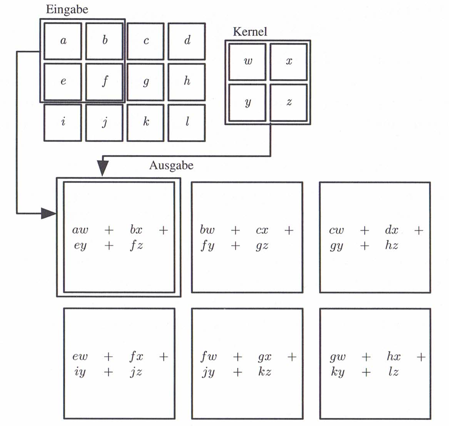
\includegraphics[scale=0.69]{Abbildungen/Anhang/Conv.png}
	\caption[Darstellung Convolutional Computation]{Darstellung der Berechnung einer 2-D-Faltung bzw. einer convolutionalen Prozedur. \cite[S. 373]{DL}}
	\label{fig:Conv2d}
\end{figure}

\subsection{Pooling Layer} \label{Pooling_Layer}
Pooling beschreibt die Minimierung der Feature Maps, wie es bereits in \ref{Conv_Layers} angesprochen wurde. Zu diesem Zweck wird in \ref{fig:Maxpool} ein Kernel und Stride der Form (2x2) gewählt, welcher ein Max-Pooling durchführen soll. Dieser Kernel bewegt sich über die Feature Map entsprechende des Strides und gibt den maximalen Wert innerhalb der Kernels wieder. Somit wird aus einer (4x4) eine (2x2) Feature Map. \cite[S. 379 ff.]{DL}

\begin{figure}[H]
	\centering
	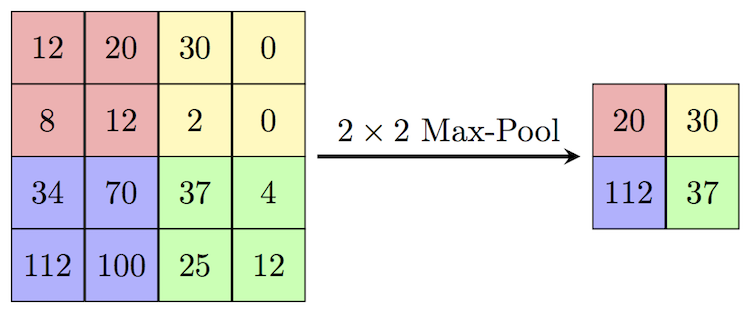
\includegraphics[scale=1.7]{Abbildungen/Anhang/Maxpool.png}
	\caption[Darstellung MaxPooling]{Darstellung des Max-Poolings. \url{https://computersciencewiki.org/images/8/8a/MaxpoolSample2.png}}
	\label{fig:Maxpool}
\end{figure}

\subsection{Fully Connected Layer} \label{FC_Layers}
Die Fully Connected Layer (FC) sind die grundlegendsten Elemente eines NN. Ein solches Layer besteht aus zwei Teilen, die beide einer Initialisierung benötigen.
Die Gewichte des FC sind als Tensor mit der Form (Anzahl der Output Features, Anzahl der Input Features) initialisiert. Zuzüglich kann optional noch ein Bias erstellt werden, welcher auf jedes Output Feature noch einen Rauschwert aufaddiert. Die Größe dieser Rauschwerte werden durch Backpropagation und Gradientenverfahren bestimmt, wie es auch bei den Gewichten der Fall ist. Die FC Layer implementieren daher folgende Funktion:
\begin{align}
	y = xA^T + b
\end{align}
wobei $y$ das Ergebnis, $x$ der Input Tensor, $A^T$ die Gewichte und $b$ das Bias, darstellt. \url{https://pytorch.org/docs/stable/generated/torch.nn.Linear.html}




\chapter{Anhang zur Implementierung}

\section{AV-Network} \label{sec:Anhang_AV_Network}
Mithilfe der Module, kann eine neues NN-Element erstellt werden.
Es wurde daher die Klasse AV\_NET definiert, welche zugleich als NN-Element benutzt werden kann.
\begin{lstlisting}[caption=Implementierung des AV-NET, style=Python]
class AV_NET(nn.Module):
	def __init__(self):
		super(AV_NET, self).__init__()
		self.AV_NET = nn.Sequential(
		nn.Conv2d(in_channels=6, out_channels=8, \
		kernel_size=(3, 3), stride=(1, 1), padding=(1, 1)),
		nn.ReLU(),
		nn.Conv2d(in_channels=8, out_channels=8, \
		 kernel_size=(3, 3), stride=(1, 1), padding=(1, 1)),
		nn.ReLU(),
		nn.ZeroPad2d((0, 1, 0, 1)),
		nn.MaxPool2d(kernel_size=2, stride=2),
		nn.Flatten(),
		nn.Linear(392, 256),
		nn.ReLU(),
		nn.Linear(256, 128)
		)
	def forward(self, av):
		return self.AV_NET(av)
\end{lstlisting}
Diese besteht aus zwei Convolutional (Conv2d), einem Max-Pooling und zwei Fully Connected Layers (Linear). 
Zwischen den Layers finden weitere Transformationen statt, welche in \autoref{subsec:Konzept_Netzstruktur} erklärt wurden.
Jedes NN-Element muss zwingend eine forward Methode implementieren, um die Propagierung der Input-Daten durch das Netzwerk zu steuern. Aus diesem Grund existiert eine forward Methode für diese Klasse, welche die AV (around\_view) durch die dargestellten NN-Schichten und Funktionen propagiert. Das Ergebnis wird zurückgegeben.


\chapter{Anleitung}
Zur besseren Anwendbarkeit der Software, wurden die Files main\_train und main\_play erstellt. Mit diesen kann ein Benutzer die Trainings- und Spielroutine starten. Alternativ lässt sich dies auch durch die Verwendung von Python spezifischen Entwicklungsumgebungen durchführen.\\
Zum Start des Trainings muss  main\_train mit den folgenden Parametern gestartet werden. Dabei ist jedoch zu beachten, dass je nach Algorithmus-Art unterschiedliche Parameter übergeben werden müssen. Die Algorithmus-Art wird zu diesem Zweck als erstes Startargument übergeben.

\section{PPO Train Startargumente} 
\begin{enumerate}
	\item "PPO" $\longrightarrow$ Algorithmus-Art
	\item N\_ITERATIONS (Int) $\longrightarrow$ Anzahl l der zu spielenden Spiele
	\item LR\_ACTOR (Float) $\longrightarrow$ Lernrate der Actor-NN
	\item LR\_CRITIC (Float) $\longrightarrow$ Lernrate des Critic-NN
	\item GAMMA (Float) $\longrightarrow$ Abzinsungsfaktor \ref{sign:Gamma}
	\item K\_EPOCHS (Int) $\longrightarrow$ Gibt die Anzahl der  Lernzyklen eines Batches bzw. Spieles an. Siehe \ref{sec:PPO_Algorithmus}
	\item EPS\_CLIP (Float) $\longrightarrow$ Clip Faktor, welcher St Standard bei 0.2. Siehe \ref{sec:PPO_Training_Objective_Function}
	\item BOARD\_SIZE (Tuple of Ints) $\longrightarrow$ Spielfeldgröße bzw. Spielfeldform. Z.B. "(8, 8)"
	\item PATH (String) $\longrightarrow$ Path an dessen Stelle ein neuer Ordner erstellt wird mit dem erlernten Modell sowie der Trainingsstatistik und den Trainingsdaten. Wenn der Standard Path verwendet werden soll: "" übergeben.
	\item DO\_TOTAL\_RUN (Boolean) $\longrightarrow$ Wenn False, wird nur bis zu dem Zeitpunkt gelernt, an dem der Agent unter den zehn letzten Spielen sechs Siege erreichen hat. Ansonsten wird ein kompletter Trainingsrun durchgeführt.
	\item GPU (Boolean) $\longrightarrow$ Wenn True und eine CUDA-fähige Grafikkarte vorhanden ist, wird der Trainingsprozess auf der Grafikkarte ausgeführt.
\end{enumerate}
So könnte ein Start mittels Kommandozeile aussehen:
\begin{center}
	Path\_to\_File\textbackslash Bachelor-Snake-AI\textbackslash src\textbackslash python main\_train.py "PPO"{} 30000 0.0001 0.0004 0.95 10 0.2 "(8, 8)"{} ""{} False True
\end{center}

\section{DQN Train Startargumente}
\begin{enumerate}
	\item "DQN" $\longrightarrow$ Algorithmus-Art
	\item N\_ITERATIONS (Int) $\longrightarrow$ Anzahl l der zu spielenden Spiele
	\item LR (Float) $\longrightarrow$ Lernrate der Q-NN
	\item GAMMA (Float) $\longrightarrow$ Abzinsungsfaktor \ref{sign:Gamma}
	\item BATCH\_SIZE (Int) $\longrightarrow$ Größe des zu entnehmenden Batches \ref{alg:DQN}
	\item MAX\_MEM\_SIZE (Int) $\longrightarrow$ Maximale Größe des Memory.
	\item EPS\_DEC (Float) $\longrightarrow$ Der Absenkungsfaktor von Epsilon \ref{alg:DQN}
	\item EPS\_END (Float) $\longrightarrow$ Der Endwert von Epsilon \ref{alg:DQN}
	\item BOARD\_SIZE (Tuple of Ints) $\longrightarrow$ Spielfeldgröße bzw. Spielfeldform. Z.B. "(8, 8)"
	\item PATH (String) $\longrightarrow$ Path an dessen Stelle ein neuer Ordner erstellt wird mit dem erlernten Modell sowie der Trainingsstatistik und den Trainingsdaten. Wenn der Standard Path verwendet werden soll: "" übergeben.
	\item DO\_TOTAL\_RUN (Boolean) $\longrightarrow$ Wenn False, wird nur bis zu dem Zeitpunkt gelernt, an dem der Agent unter den zehn letzten Spielen sechs Siege erreichen hat. Ansonsten wird ein kompletter Trainingsrun durchgeführt.
	\item GPU (Boolean) $\longrightarrow$ Wenn True und eine CUDA-fähige Grafikkarte vorhanden ist, wird der Trainingsprozess auf der Grafikkarte ausgeführt.
\end{enumerate}
So könnte ein Start mittels Kommandozeile aussehen:
\begin{center}
	Path\_to\_File\textbackslash Bachelor-Snake-AI\textbackslash src\textbackslash python main\_train.py "DQN"{} 30000 0.0001 0.99 64 2048 0.00007 0.01 "(8, 8)"{} ""{} False True
\end{center}

\section{Play Startargumente}
Da die Play Methoden der beiden Algorithmus-Arten nahe zu identisch sind, teilen sie alle Startargumente bis auf die Algorithmus-Art. Daher können die Startparameter beider Methoden zusammen erklärt werden.
\begin{enumerate}
	\item "DQN" / "PPO" $\longrightarrow$ Algorithmus-Art	
	\item PATH (String) $\longrightarrow$ Path der Model Datei.
	\item N\_ITERATIONS (Int) $\longrightarrow$ Anzahl l der zu spielenden Spiele.
	\item BOARD\_SIZE (Tuple of Ints) $\longrightarrow$ Spielfeldgröße bzw. Spielfeldform. Z.B. "(8, 8)"
	\item PRINT\_STATS (Boolean) $\longrightarrow$ Wenn True, werden Informationen über den abgeschlossen Spielverlauf auf der Konsole erscheinen.
	\item HAS\_GUI (Boolean) $\longrightarrow$ WENN True wird die GUI \ref{sec:Impl_GUI} dargestellt.
	\item GPU (Boolean) $\longrightarrow$ Wenn True und eine CUDA-fähige Grafikkarte vorhanden ist, wird der Spielprozess auf der Grafikkarte ausgeführt.
\end{enumerate}
So könnte ein Start mittels Kommandozeile aussehen:
\begin{center}
	Path\_to\_File\textbackslash Bachelor-Snake-AI\textbackslash src\textbackslash python main\_play.py "PPO"{} "Path\_to\_Model"{} 300 "(8, 8)"{} True True True
\end{center}

%-------------
%---Schluss---
%-------------

\backmatter %Keine nummerierten Kapitel für z.B. Glossar, Index, Erklärung, etc.

\pagenumbering{gobble} %keine Seitenzahl auf der Erklärung
\chapter*{Erklärung}
Hiermit versichere ich, \autor{}, dass ich diese Arbeit selbständig verfasst und keine anderen als die angegebenen Quellen und Hilfsmittel benutzt habe. Außerdem versichere ich, dass ich die allgemeinen Prinzipien wissenschaftlicher Arbeit und Veröffentlichung, wie sie in den Leitlinien guter wissenschaftlicher Praxis der \universitaet{} festgelegt sind, befolgt habe.

\vspace{3cm}

{\def\arraystretch{2}
\begin{tabular}{p{8cm}}
\hline 
\autor \\ 
\end{tabular}
}

 %Erklärung auf der letzten Seite der gesamten Arbeit



\end{document}